\documentclass[journal]{IEEEtran}

\usepackage{amsmath,amssymb,amsfonts}
\usepackage{booktabs}
\usepackage{cite}
\usepackage{graphicx}
\usepackage{algorithm}
\usepackage{algpseudocode}
\floatstyle{plaintop}
\restylefloat{algorithm}
\usepackage{array}
\usepackage{url}
\makeatletter
\setlength{\@fptop}{0pt}
\setlength{\@fpsep}{12pt}
\setlength{\@fpbot}{0pt plus 1fil}
\setlength{\@dblfptop}{0pt}
\setlength{\@dblfpsep}{12pt}
\setlength{\@dblfpbot}{0pt plus 1fil}
\newcommand{\RestoreBibliographyColumns}{%
\clearpage
\global\@colht\textheight
\global\@colroom\textheight
\global\vsize\textheight}
\makeatother
\newcommand{\AITextRef}{\textsuperscript{\ref{fn:ai-text}}}

\title{Transition Based Closed Loop Restoration for Mobility Coupled Distribution Systems with Executable Actions}

\author{Weian~Guo, Jun~Min, and Wuzhao~Li%
\thanks{Weian Guo is with the Sino-German College of Applied Sciences, Tongji
University, Shanghai, China, email guoweian@tongji.edu.cn.}%
\thanks{Jun Min is with the College of Information Engineering, China Jiliang
University, Hangzhou, Zhejiang, China, email minjun@cjlu.edu.cn.}%
\thanks{Wuzhao Li is with Wenzhou Polytechnic, Wenzhou, Zhejiang, China, 310000,
email lwzhao055@wzpt.edu.cn. Corresponding author is Wuzhao Li.}}

\begin{document}
\maketitle

\begin{abstract}
Restoration in mobility coupled distribution systems requires charging,
communication, and repair decisions that remain feasible after network and
crew constraints are applied.  This paper develops physically constrained
coupled rollout with reference protection.  Candidate repair routes are
compared by predicted service cost against the same executable reference
across plausible transition models.  Insufficient predicted advantage retains
the reference route.  Continuous allocations use observed history and shared
demand forecasts, while packet delivery, electrical feasibility, and crew
completion determine realized service.  The analysis establishes continuous
sensitivity, conditional route regret, relative protection under a differential
error condition, and execution constraints.  Measured electric vehicle
charging, public outage observations, and an independent feeder support
paired comparisons.  Service cost evaluation improves on exposure scores.
Adding threat propagation gives a smaller average benefit over the same
service score without propagation.  Reference protection retains most of
this benefit while reducing additional losses under parameter misspecification.
Independent municipal charging inputs support the fixed comparison, with
benefits distinct from uniform superiority in total-cost tails.  The resulting
service restoration model connects distribution systems, communication
networks, and crew routing through explicit decisions and completion events.
\end{abstract}

\begin{IEEEkeywords}
service restoration, electric vehicle charging, distribution systems,
communication networks, crew routing.
\end{IEEEkeywords}

\section{Introduction}
\label{sec:introduction}

Electric vehicles connect urban travel with distribution system operation.\footnote{\label{fn:ai-text}OpenAI Codex assisted with text revision, mathematical exposition, and computational scripts. The tool provider is OpenAI, \url{https://openai.com/}.}
Charging demand moves with daily activity, station access, road conditions, and
driver choice.  Its spatial pattern therefore differs from a conventional
fixed load profile.  Station planning and traffic power flow studies have shown
that route choice and charging capacity can alter both travel and electrical
states \cite{he2015charging,wei2018trafficpower,qian2021fast}.  Operational
pricing and navigation models extend this relation to real time charging
decisions \cite{cui2021pricing,li2024inverse,ran2024fast}.  During a disruptive
event, however, demand movement is only one part of the problem.  Charging
service also depends on feeder margin, communication availability, and the time
at which a repair crew completes its work.

These dependencies give restoration a temporal and cross domain structure.
Communication supports sensing, charging coordination, and control delivery.
Loss of local power may reduce that service after backup supply is exhausted.
Delayed communication can then restrict charging actions and increase backlog.
Road disruption can move demand toward stations whose electrical capacity is
already scarce.  Interdependent infrastructure studies explain why failures
can spread across connected services \cite{rinaldi2001interdependencies,
ouyang2014review}.  Power system resilience research further relates
restoration decisions to service continuity under uncertain events
\cite{panteli2015resilience,ti2022resilience}.  The resulting decision cannot be
reduced to repairing the zone with the largest current loss because a moderate
present threat may lie on a more consequential future path.

Demand forecasts provide useful information for this decision.  Recent graph
models represent spatial dependence and recurring temporal behavior in traffic
series \cite{yin2022deep,jiang2023survey}.  Several
models improve prediction under changing graph relations and limited
observations \cite{jin2023autodstsgn,li2023few,shin2024pgcn}.  Prediction error
alone does not determine restoration quality.  Two policies can receive the
same forecast and still choose different actions because only one evaluates
the propagation of road, power, and communication threats.  Digital
representations of physical operation provide a natural setting for this
evaluation when their variables correspond to service and network constraints
\cite{tao2019digital,fuller2020digital,minerva2020digital}.

A further distinction concerns the quantity used to compare repair plans.
Accumulated threat exposure can identify a heavily affected zone, but it does
not directly specify the service recovered by completing a repair there.  That
service depends on the demand remaining when the crew finishes, available
charging and communication resources, and backlog carried from earlier hours.
Two routes can therefore have similar exposure scores but different service
costs.  A decision rule should compare their completion schedules through the
same service equations used to value an action.  Its evaluation should then
separate the effect of that service objective from the additional effect of
predicting propagation.  This distinction also determines the mathematical
object of interest.  Continuous priorities admit sensitivity analysis, whereas
selecting one integer route from a finite set calls for a comparison of route
scores and realized costs.

The present study addresses three connected decisions.  The first is the
conversion of a shared demand forecast into a finite horizon restoration score
that includes action dependent threat propagation.  The second is the
conversion of continuous service priorities into actions that satisfy packet,
feeder, station, and crew constraints.  The third is the separation between a
predictive repair priority and the integer completion event that actually
changes the state.  Treating a requested priority as completed repair would
credit service before a crew arrives.  Treating an unprojected charging request
as served load would create the same inconsistency on the electrical side.

This paper develops physically constrained coupled rollout, abbreviated as PC
rollout.  A compact graph recurrent model forecasts station arrivals and
charging energy.  A nonnegative transition model propagates mobility, power,
and communication threats over a finite horizon.  Central PC evaluates each
candidate under the calibrated central transition, while a robust extension
minimizes the worst absolute score over a declared finite matrix set.
PC with reference protection instead compares each route with the same
executable reference under each matrix and retains that reference when the
predicted advantage is insufficient.  This distinguishes protection against
a harmful replacement from minimizing the largest absolute cost.
Requested charging and communication actions are reduced when
packets miss their deadlines.  Charging is then projected through an
independent SMART-DS and OpenDSS calculation.  Repair priorities form work
orders, integer crew routes, and recorded completion events.  Only executable
service and completed repair enter the next realized state.

The paper makes the following theoretical and algorithmic contributions.
\begin{itemize}
\item It formulates an action dependent finite horizon restoration rule that
selects a committed repair route by predicted service losses and backlog.
A paired comparison across transition models protects an executable reference
when a replacement has insufficient predicted advantage.  Continuous service
allocations are recalculated as new observations arrive.
\item It constructs an executable action algorithm that distinguishes requested
service, packet delivery, distribution system projection, dispatched work
orders, and integer repair completion.  A capacity constrained assignment model
treats station reassignment separately.
\item It establishes finite horizon sensitivity for the continuous prediction
and allocation layer, conditional regret and reference protection bounds for
finite route selection, and feasibility and invariance results for executed
actions.
\end{itemize}

The rest of this paper is organized as follows.  Section II reviews related
work.  Section III presents the system model, decision rule, and mathematical
results.  Section IV presents the empirical study, interprets the evidence, and
states data availability.  Section V concludes the paper.

\section{Related Work}
\label{sec:related}

\subsection{Electric mobility and distribution grids}

Electric mobility couples travel activity with distribution system operation.\AITextRef
Charging deployment models connect station access and trip demand with
infrastructure placement \cite{he2015charging,sadeghi2014fast}.
Stochastic demand models describe uncertainty and flexibility in vehicle
charging \cite{alizadeh2014pev}.  Later planning studies incorporate road
traffic uncertainty \cite{deb2022charging} and coordinate investments in
roads, charging stations, and distribution networks \cite{li2023milp}.  Extreme
fast charging models add demanding electrical constraints to station location
and service design \cite{qian2021fast}.  Traffic power flow formulations place
route decisions and distribution constraints in a common optimization model
\cite{wei2018trafficpower,lv2020semidynamic}.  This literature establishes the
physical relation between mobility and charging load.

Operational studies move the decision from capacity planning to traveler and
station control.  Pricing and navigation coordinate route choice with charging
availability and distribution states \cite{cui2021pricing,li2024inverse,
ran2024fast}.  Distributed assignment has also been studied when information
and control are exchanged across cyber physical components
\cite{tao2024distributed}.  These charging models decide capacity, prices, or
routes.  Restoration introduces an additional time
sequence because communication delivery, feeder feasibility, and crew
completion determine when a requested action becomes effective.

The timing distinction changes the mathematical role of an action.  In a
planning model, installed capacity is available once the investment decision is
made.  In a navigation model, a recommended route can enter the traffic state
within the next assignment interval.  A restoration request instead passes
through message delivery, travel, and service before it changes local
conditions.  Charging coordination studies provide the demand and network
relations needed for this setting \cite{cui2021pricing,tao2024distributed}.
They leave room for an event based state update that records service only after
the corresponding electrical or crew condition has been met.

\subsection{Cyber physical resilience and digital twins}

Interdependent infrastructure theory describes failure transfer across network
layers and the resulting service consequences
\cite{rinaldi2001interdependencies,ouyang2014review}.  Network models show that
coupled systems can develop abrupt cascades \cite{buldyrev2010cascade}.
Spreading process analysis supplies tools for studying the growth and control of
such dynamics on graphs \cite{nowzari2016epidemics}.  Power system resilience
research relates these dependencies to service continuity under extreme events
\cite{panteli2015resilience}.  Proactive recovery models coordinate crew
mobilization before a hurricane with equipment repair after the event
\cite{arab2015proactive}.  Coupled power and information models also include
communication traffic constraints and collaborative recovery under typhoon
damage \cite{ti2022resilience}.  Restoration and communication dependent
recovery therefore precede the present study.  Its focus is their connection
to charging service costs, predicted threat propagation, and recorded crew
completion.  Reinforcement learning offers a related approach to
sequential decisions in transportation systems \cite{haydari2020rl}.  The present model uses
this temporal view but keeps the action mechanism explicit so that a repair
priority and a completed repair remain different states.

Physically constrained security research considers whether learned grid
functions and adversarial inputs satisfy power balance, operating limits, and
stealth requirements.  Formal evaluation has been developed for intelligent
security assessment and tree ensemble applications
\cite{zhang2023robustness,zhang2023datasecurity}.  Hybrid learned and classical
load frequency control has also been studied under physically admissible attack
models \cite{zhang2026physicsattack}.  Those studies constrain cyber security
analysis with grid equations.  The restoration problem here instead allocates
charging, communication, and repair resources over time, then subjects each
request to physical and operational execution rules.

Digital representations provide a related basis for testing a decision before
it is applied.  General studies define the connection among a physical asset,
its computational representation, and data exchange
\cite{tao2019digital,fuller2020digital}.  Networked and industrial models stress
the need for an operational relation between the representation and the asset
\cite{minerva2020digital,ding2021digital}.  The model in this paper represents
charging service, backlog, communication capacity, threat propagation, feeder
feasibility, and crew progress.  These variables are used to calculate an
action and its realized consequences rather than to create a visual copy of the
system.

This operational use requires consistent clocks across the represented
services.  Demand and threat are observed at the decision interval.  Packet
events occur within that interval.  Crew travel and repair can continue across
several intervals.  A continuous simulator can rank candidate actions, while
the realized state must wait for the discrete event that makes the action
effective.  Digital representation studies support the connection between
physical state and computational state \cite{fuller2020digital,
minerva2020digital}.  The present formulation uses that connection to separate
the predictive state from the executed state and to keep their update rules
explicit.

Comparing a proposed decision with a common reference also has an established
role in optimization under model uncertainty.  Robust baseline regret
evaluates both policies under the same transition model before taking the
adverse model choice \cite{petrik2016baseline}.  That work studies discounted
Markov policies and the complexity of their optimization.  Here the decision
is a finite, committed crew route with explicit completion times.  Reference
protection specializes the comparison to predicted service costs and adds a
fixed acceptance margin.  Its execution bound depends on the error in route
cost differences, separately from continuous forecast sensitivity.

\subsection{Graph forecasting for charging states}

Charging forecasts estimate when and where vehicles will request service.
Reviews describe the spatial and temporal structures used in traffic
prediction \cite{jiang2023survey,rahmani2023gnnits,yin2022deep}.
Automated graph construction represents relationships that vary across time
and data sets \cite{jin2023autodstsgn}.  Fast spatiotemporal learning combines
efficient graph operations with temporal information at several scales
\cite{guo2023fast}.  LocaleGN uses local traffic relationships to learn from
few observations and transfer predictions across cities \cite{li2023few}.
Self supervision and self distillation use temporal context to improve
generalization \cite{ji2023self}.  Progressive graph convolution adapts spatial
relations during both training and prediction \cite{shin2024pgcn}.  Direct
measurement studies nevertheless show that charging behavior retains substantial
spatial and temporal variation \cite{martz2022charging}.

Most forecasting models optimize prediction error, whereas restoration depends
on the decision induced by a forecast.  A forecast can have low average error
and still assign insufficient attention to a zone on a future propagation path.
The forecaster in this paper is therefore a shared state estimator.  Central PC
and the forecast matched baseline receive the same forecast, current threat,
backlog, and realized history.  Their difference is the propagation calculation
used to value a candidate route.  This comparison isolates the transition model
from demand prediction and preserves equal information at the decision time.

Public infrastructure data also have distinct evidentiary roles.  Measured
charging transactions provide station demand.  County outage observations
provide temporal information about power events \cite{brelsford2024eaglei}.
An independent distribution feeder determines whether a charging request is
electrically feasible.  Keeping these roles separate avoids representing
records from different systems as one geographically coincident network.  The
method joins them through stated model variables.  Charging requests and crew
orders pass through packet, feeder, and completion checks.  Station
reassignment is evaluated separately under capacity constraints.

The literature therefore supplies four strands of the present problem.
Charging studies describe demand movement and service capacity.  Infrastructure
resilience studies describe propagation across connected domains.  Graph
forecasting estimates the near future demand state.  Digital representations
connect a candidate decision to operational constraints.  The present
algorithm combines these strands through a common information set and an
event based execution rule.  This combination permits a direct comparison
between transition evaluation and a baseline that receives the same forecast
without using the transition model.

\section{System Model and Restoration Method}
\label{sec:method}

\subsection{Operating state}
\label{sec:state}

Let $G=(V,E)$ be a charging service graph with $N$ station zones.\AITextRef\ Each station
is linked to its four geographically nearest neighbours.  Symmetrizing this
neighbour relation, applying Gaussian distance weights, and adding self links
gives $W$.  Its row normalization is $A$.  The realized service state during
hour $t$ is
\begin{equation}
x_t=(m_t,e_t,q_t),
\end{equation}
where $m_t\in\mathbb{R}_+^N$ is mobility activity that drives charging demand,
$e_t\in\mathbb{R}_+^N$ is charging energy demand, $q_t\in\mathbb{R}_+^N$ is
charging backlog.  Communication load and feeder load are calculated from the
current service request.  The separate state $z_t=(z_t^r,z_t^p,z_t^c)$ is the
mobility, power, and communication threat field.  Each threat field lies in
$[0,1]^N$.  It is a normalized service degradation intensity, not the binary
state of one breaker, line, or router.  For example, $z_i^p=0.6$ means a 60\%
derating in the zone level power dependent service factor.  The value
$z_i^r=0.6$ produces
a 60\% proportional mobility impairment before the communication term.  A
binary outage can be represented as a high intensity limiting case.  The
scenario scope includes cyber induced loss of sensing and control availability and
physical or service failures.  The state describes service degradation without
assigning a particular attack type.  Before choosing an action for hour $t$,
the controller observes backlog, threat, and charging history through hour
$t-1$.  Current arrival demand is evaluated after that action is requested.
The controller therefore uses the forecast state
$\hat x_t=(\hat m_t,\hat e_t,q_t)$ and the shared forecast continuation, rather
than the future realized demand in $x_t$.

The requested decision is
\begin{equation}
a_t=(u_t^{\mathrm{ch}},u_t^{\mathrm{com}},u_t^{\mathrm{res}}).
\end{equation}
The first term allocates charging service capacity, the second allocates
communication service capacity, and the third is a continuous restoration
priority used by the predictive scoring layer.  It is not itself a completed
repair.
The feasible set is
\begin{equation}
\begin{aligned}
\mathcal{A}=\{a_t\ge0 \mid&
\mathbf{1}^{\top}u_t^{\mathrm{ch}}\le B_{\mathrm{ch}},\\
&\mathbf{1}^{\top}u_t^{\mathrm{com}}\le B_{\mathrm{com}},\\
&\mathbf{1}^{\top}u_t^{\mathrm{res}}\le B_{\mathrm{res}}\}.
\end{aligned}
\end{equation}
Here $B_{\mathrm{ch}}$, $B_{\mathrm{com}}$, and $B_{\mathrm{res}}$ are the
available charging, communication, and normalized restoration resources during
one decision interval.  The continuous restoration variable is a service level
priority used to order a common set of work orders.  Integer crews follow
explicit routes with travel times, service times, and recorded repair
completion events.  At every policy hour, charging action is also
projected through the SMART-DS and OpenDSS feasibility loop before service is
credited and backlog is updated.

\subsection{Grid and service equations}
\label{sec:service}

The continuous prediction layer uses service equations that are
continuous, piecewise smooth, and Lipschitz on the stated bounded domain.
The minimum, positive part, and clipping operators need not be differentiable
at their switching points.
For zone $i$ and rollout step $h$, available communication service is
\begin{equation}
\bar c_{i,h}=u_{i,h}^{\mathrm{com}}(1-z_{i,h}^{p})(1-\alpha_c z_{i,h}^{c}),
\end{equation}
where $\alpha_c\in[0,1]$ measures direct communication degradation.  The load
placed on communication is
\begin{equation}
c_{i,h}=\beta_m m_{i,h}+\beta_e(e_{i,h}+\rho_q q_{i,h})
+\beta_r z_{i,h}^{r}+\beta_p z_{i,h}^{p}.
\end{equation}
The resulting communication loss is
\begin{equation}
\ell_{i,h}^{c}=[c_{i,h}-\bar c_{i,h}]_+.
\end{equation}
Communication support affects charging coordination and mobility service through
\begin{equation}
\eta_{i,h}^{c}=1-\min\left\{0.9,\frac{\ell_{i,h}^{c}}{1+c_{i,h}}\right\}.
\end{equation}
This algebraic relation is an hourly workload model.  Executability is supplied
by a finite buffer packet emulator with retransmission and deadline logic.  If
$d_{i,h}\in[0,1]$ is the simulated fraction of control packets delivered before
their deadline, the delivered charging and communication requests are
\begin{equation}
\tilde u_{i,h}^{k}=d_{i,h}u_{i,h}^{k},\qquad
k\in\{\mathrm{ch},\mathrm{com}\}.
\label{eq:packet-derate}
\end{equation}
The emulator keeps full service rate while backup power is available and
applies power induced service derating only after backup exhaustion.  Packet
loss and delay therefore change the implemented action rather than appearing
only as a later diagnostic.  For each station, traffic multiplier, and backup
duration, the main loop reads the closest simulated power and communication
threat pair from a fixed response table.  Squared distances use scales 0.75 and
0.375 for the two threat coordinates.  This table is generated from training
period activity before the validation and test experiments.  It supplies packet
execution fractions without fitting a queue model to test outcomes.
In execution, communication support is evaluated with
$\tilde u^{\mathrm{com}}$ in place of $u^{\mathrm{com}}$.  The resulting raw
charging service $r_h$ is mapped to three phase SMART-DS loads.  Bisection
retains a tested feasible fraction $\alpha_h^{\mathrm{AC}}\in[0,1]$, giving
\begin{equation}
s_{i,h}^{\mathrm{ch}}=\alpha_h^{\mathrm{AC}}r_{i,h}.
\label{eq:smartds-project}
\end{equation}
The feeder must converge, voltages at nodes energized in the released base case must lie in
$[0.95,1.05]$ p.u., and maximum line loading must not exceed 1.0 p.u.  Charging
service before electrical projection is
\begin{equation}
r_{i,h}=
\min\left\{e_{i,h}+\rho_q q_{i,h},
\tilde u_{i,h}^{\mathrm{ch}}(1-z_{i,h}^{p})\eta_{i,h}^{c}\right\}.
\end{equation}
The charging backlog evolves as
\begin{equation}
q_{i,h+1}=
\left[e_{i,h}+\rho_q q_{i,h}
-s_{i,h}^{\mathrm{ch}}\right]_+ .
\end{equation}
We impose $0\le\rho_q<1$ and set $\rho_q=0.22$.  If hourly
arrival energy is bounded by $\bar e$, then
$q_{i,h+1}\le \bar e+\rho_q q_{i,h}$ and consequently
$q_{i,h}\le\max\{q_{i,0},\bar e/(1-\rho_q)\}$.

Electrical outcomes are the solved node voltages and line loadings, rather than
the earlier scalar feeder margin.  Executable charging is determined by
\eqref{eq:smartds-project}.
The demand weighted mobility loss is
\begin{equation}
\ell_{i,h}^{m}=
m_{i,h}\left(z_{i,h}^{r}+\beta_{mc}(1-\eta_{i,h}^{c})\right).
\end{equation}
Unserved charging is defined once as
$\ell_{i,h}^{e}=[e_{i,h}+\rho_q q_{i,h}-s_{i,h}^{\mathrm{ch}}]_+$, and
power dependent service loss is
$\ell_{i,h}^{p}=z_{i,h}^{p}(e_{i,h}+\rho_q q_{i,h})$.
The coefficients in these equations have fixed physical roles.  The parameters
$\beta_m$, $\beta_e$, $\beta_r$, and $\beta_p$ convert mobility activity,
charging demand, mobility threat, and power threat into communication workload.
The coefficient $\rho_q$ is backlog carryover, while $1-z^p$ represents power
availability.  The coefficient $\beta_{mc}$ converts
communication service reduction into delayed trip equivalents.
Here a trip equivalent is one charging arrival weighted by the modeled service
disruption.  It is not an observed travel time or an independently measured
traffic delay.
The stage risk is
\begin{align}
L(x_h,a_h,\zeta_h)
=\sum_{i=1}^{N}\big(&
\lambda_m\ell_{i,h}^{m}+\lambda_e\ell_{i,h}^{e} \nonumber\\
&+\lambda_c\ell_{i,h}^{c}
+\lambda_p\ell_{i,h}^{p} \nonumber\\
&+\lambda_z[z_{i,h}^{p}z_{i,h}^{c}
+z_{i,h}^{r}(1-\eta_{i,h}^{c})]\big).
\label{eq:stage}
\end{align}
The nonnegative weights $\lambda_m$, $\lambda_e$, $\lambda_c$, $\lambda_p$, and
$\lambda_z$ set the relative contributions of mobility delay, unmet charging
demand, communication loss, power dependent service loss, and cross domain
exposure.  The weights carry reciprocal units for their respective losses.
Thus $\lambda_m$ is per trip equivalent, $\lambda_e$ and $\lambda_p$ are per kWh,
$\lambda_c$ is per communication workload unit, and $\lambda_z$ is dimensionless.
Their numerical values define a dimensionless comparison score, not monetary cost.
Unserved charging appears only through $\ell^e$.  All coefficients are held
fixed across policies.

For a feasible policy $\pi$, the finite horizon rollout objective at decision
time $t$ is
\begin{align}
J_H^{\pi}(x_t,\zeta_t)
&=\sum_{h=0}^{H-1}\gamma^h L(x_{t+h},a_{t+h},\zeta_{t+h}), \label{eq:objective}\\
a_{t+h}
&=\pi(\hat x_{t+h},\zeta_{t+h},A).
\end{align}
The objective in \eqref{eq:objective} sums this dimensionless stage score.
The shared forecast continuation is suppressed in the policy notation.
All reported experiments use $\gamma=1$.  Charging and communication allocations
are recalculated hourly from the new observation and the remaining episode
horizon.  Crew routes are selected at the initial dispatch and remain committed
throughout that episode.  Thus service allocation responds to subsequent
observations without assuming that a travelling crew can change its route
instantaneously.

\subsection{Demand forecasting}
\label{sec:forecast}

The forecaster estimates mobility and charging demand.
\begin{equation}
\hat y_{t,\ldots,t+H-1}=f_{\theta}(y_{t-L},\ldots,y_{t-1},A),
\end{equation}
where $y_t=(m_t,e_t)$, $L$ is the historical window, and $H$ is the rollout
horizon.  The implemented model first mixes node features through $A$, then
updates zone states using a recurrent cell, and finally maps the hidden state to
the horizon.  Keeping the forecaster small makes its role clear inside the
larger decision model.  Classical baselines and the learned model are compared
in Section IV so that the decision results can be interpreted relative to the
forecasting quality.

At the beginning of hour $t$, the last demand observation is $y_{t-1}$.
The input series is transformed by a logarithmic map and normalized using only
the training period.  For a time index $\tau$,
\begin{equation}
\tilde y_{\tau}=
\frac{\log(1+y_{\tau})-\mu}{\sigma}.
\end{equation}
The graph recurrent forecaster uses one graph mixing operation before each
recurrent update and layer normalization after it.  With hidden state
$h_{\ell}$ inside the historical window,
\begin{align}
g_{\ell} &= A\tilde y_{t-L+\ell-1},\\
h_{\ell} &= \mathrm{LN}(\mathrm{GRU}(W_g g_{\ell}+b_g,Ah_{\ell-1})),\\
o &= W_2\,\mathrm{GELU}(W_1h_L+b_1)+b_2.
\end{align}
The output is reshaped to the forecast horizon and transformed back to demand
units as $[\exp(\sigma o+\mu)-1]_+$.  Dropout is disabled during inference.  The
primary forecaster is trained with the Huber loss in normalized logarithmic
coordinates
\begin{equation}
\mathcal{L}_{\mathrm{for}}=\mathcal{L}_{\mathrm{Huber}}(o,\tilde y).
\end{equation}
Its spatial inductive bias comes from the fixed station distance graph mixing
inside the recurrent model, not from an additional physical penalty.
Three independent training runs are performed, and the model retained for the
decision study is selected only by its validation score.  Every training target
lies within the training period, and every validation target lies within the
validation period.  No target window crosses either calendar boundary.

\subsection{Transition model and action construction}
\label{sec:construction}

Let $\zeta_h=(z_h^r,z_h^p,z_h^c)\in[0,1]^{3N}$.  Two transitions are kept
explicit because prediction and execution have different roles.  The
continuous transition used only to score the requested restoration priority
$u^{\rm pri}=u^{\rm res}$ is
\begin{equation}
\hat\zeta_{h+1}=
\Pi_{\mathcal{Z}}\left(M\hat\zeta_h-R\psi(u_h^{\mathrm{pri}})+\hat\xi_h\right),
\label{eq:propagation}
\end{equation}
where $\mathcal{Z}=[0,0.98]^{3N}$, $\Pi_{\mathcal{Z}}$ is Euclidean projection,
$M\ge0$ is the cross domain propagation matrix, and $R\ge0$ stacks the three
domain repair coefficients.  The implemented saturation is
$\psi_i(u)=\min\{3,[u_i/\delta]_+\}$, where $\delta$ is the per zone reference
resource.  Thus $\psi$ is $1/\delta$ Lipschitz.  The scorer assumes
$\hat\xi_h=0$ for deployable policies.  Equation
\eqref{eq:propagation} does not update the realized state.

For execution, let $\bar r_{i,h}\in\{0,1\}$ indicate that a dispatched work
order in zone $i$ has completed by the end of interval $h$, and define
$D(\bar r_h)=I_3\otimes\operatorname{diag}(1-\bar r_h)$.  The main simulator
uses
\begin{equation}
\zeta_{h+1}=D(\bar r_h)
\Pi_{\mathcal Z}\left(M\zeta_h+\xi_h\right).
\label{eq:executed-propagation}
\end{equation}
Waiting, travel, and service do not change $\bar r_h$.  Only a recorded crew
completion event changes it from zero to one.  Thus no continuous priority is
credited as realized repair.  With
$K_d=\rho_dI+\sigma A$ for $d\in\{r,p,c\}$, the implemented matrix is
\begin{equation}
M=\begin{bmatrix}
K_r&\tau_{pr}I&\tau_{cr}I\\
0&K_p&\tau_{cp}A\\
\tau_{rc}A&\tau_{pc}I&K_c
\end{bmatrix}.
\label{eq:Mblocks}
\end{equation}
The block structure in \eqref{eq:Mblocks} separates persistence, spatial
spread, and directed cross domain effects.  The normalized adjacency $A$
enters both within domain spread and selected
cross domain paths.  Boulder charging deficits estimate $\rho_r$ and $\sigma$.
EAGLE-I Boulder County outages estimate $\rho_p$.  Aligned outage and charging
records bound $\tau_{pr}$.  The packet emulator constructs the
power to communication interval for $\tau_{pc}$.  Coefficients lacking joint
field observations are assigned sensitivity ranges.  Bootstrap and
sign constrained intervals define an uncertainty set $\mathcal U$.  The central
matrix has spectral radius 1.062 and Euclidean operator norm 1.176, so no asymptotic contraction is
claimed.  Projection makes the implemented state set invariant and the policy is
evaluated over a finite six hour horizon and a 100,000 step stress test.

PC rollout scores restoration by its action dependent marginal benefit.  Let
$w_{i,h}$ be a bounded exposure weight formed from the shared mobility and
energy forecast, and let $\Omega=\mathrm{diag}(\omega_r,\omega_p,\omega_c)$.
For a candidate first restoration vector $v$, define
\begin{equation}
\mathcal{C}_t(v)=\sum_{h=0}^{H-1}\sum_{i=1}^{N}
 w_{i,h}\mathbf{1}^{\top}\Omega\hat\zeta_{i,t+h}(v),
\label{eq:envelope}
\end{equation}
where $\hat\zeta_{t+h}(v)$ follows \eqref{eq:propagation}, using $v$ only in the
first predicted transition.  For reference quantum $\delta$, the marginal
benefit of repairing zone $i$ is
$b_{i,t}(M)=[\mathcal{C}_t(0,M)-\mathcal{C}_t(\delta e_i,M)]_+$.  The primary
policy uses the calibrated central matrix $M_c$,
$b_{i,t}^{\rm cen}=b_{i,t}(M_c)$.  A separately evaluated robust extension uses
the lower envelope
\begin{equation}
b_{i,t}^{\rm rob}=\min_{M\in\mathcal U_V} b_{i,t}(M),
\end{equation}
where $\mathcal U_V$ contains the central matrix, joint lower and upper
vertices, and the endpoints of each individual coefficient (21 matrices in the
tested set).  The policy specific time indexed restoration score is
\begin{equation}
s_{i,t}^{\mathrm{res}}=
\omega_pz_{i,t}^{p}+\omega_cz_{i,t}^{c}+\omega_rz_{i,t}^{r}
+\omega_{\Gamma}b_{i,t}^{\pi}.
\end{equation}
Here $b^{\pi}=b^{\rm cen}$ for central PC candidate construction and
$b^{\pi}=b^{\rm rob}$ only for the robust extension.
The restoration action uses a small uniform reserve and a concave risk
allocation.
\begin{equation}
u_i^{\mathrm{res}}=
\frac{\eta B_{\mathrm{res}}}{N}
+(1-\eta)B_{\mathrm{res}}
\frac{\sqrt{s_i^{\mathrm{res}}+\epsilon}}
{\sum_{j=1}^{N}\sqrt{s_j^{\mathrm{res}}+\epsilon}},
\label{eq:allocation}
\end{equation}
where $0\le\eta\le1$ is the reserve fraction.  The square root reduces
allocation contrasts relative to proportional weighting of the same positive
scores.  The reserve gives every zone at least $\eta B_{\rm res}/N$ without
imposing an additional cap on a high priority zone.
The weights $\omega_p$, $\omega_c$, $\omega_r$, and $\omega_{\Gamma}$ are
nonnegative constants that control direct domain exposure and the multistep
action benefit.  The constant $\epsilon$ is a small positive stabilizer that
keeps every zone eligible for a nonzero reserve.

Charging and communication capacities are assigned with the same allocator so
that all resource decisions share the same feasibility structure.  For any
budget $B\ge0$, nonnegative score vector $v$, and reserve fraction
$\eta_B\in[0,1]$, define
\begin{equation}
\Phi_i(B,v,\eta_B)=
\frac{\eta_B B}{N}
+(1-\eta_B)B
\frac{\sqrt{v_i+\epsilon}}
{\sum_{j=1}^{N}\sqrt{v_j+\epsilon}}.
\label{eq:allocator}
\end{equation}
PC rollout uses
\begin{align}
u_i^{\mathrm{ch}}&=\Phi_i(B_{\mathrm{ch}},g^{\mathrm{ch}},\eta_{\mathrm{ch}}),\\
u_i^{\mathrm{com}}&=\Phi_i(B_{\mathrm{com}},g^{\mathrm{com}},\eta_{\mathrm{com}}),
\end{align}
where
\begin{align}
g_{i,t}^{\mathrm{ch}}
&=\sum_{h=0}^{H-1}\hat e_{i,t+h}+\kappa_q q_{i,t}
+\kappa_{\mathrm{ch}}
\left(z_{i,t}^{r}+z_{i,t}^{p}+z_{i,t}^{c}\right),\\
g_{i,t}^{\mathrm{com}}
&=\sum_{h=0}^{H-1}\hat m_{i,t+h}
+\kappa_E\left(\sum_{h=0}^{H-1}\hat e_{i,t+h}+\kappa_q q_{i,t}\right) \nonumber\\
&\quad+\kappa_{\mathrm{com}}
\left(z_{i,t}^{r}+z_{i,t}^{p}+z_{i,t}^{c}\right).
\end{align}
Service capacity follows predicted demand, while the requested restoration
priority follows the future cascade envelope.  Charging and communication
resources serve expected load.  In the scoring layer, priority perturbs
\eqref{eq:propagation}.  In the execution layer, only the completion indicator
in \eqref{eq:executed-propagation} changes realized threat.
The coefficients $\kappa_q$, $\kappa_{\mathrm{ch}}$, $\kappa_E$, and
$\kappa_{\mathrm{com}}$ determine how observed backlog, current threat, and
forecasted charging demand alter the time varying service scores.  For the main
experiment, an initial threat realization and adjacency based propagation
create a policy independent set of at most 36 work orders.  Four integer crews
start from a common depot.  Candidate routes are constructed from static,
greedy, forecast matched, central PC, robust PC, and uniform priorities using
the same jobs, travel matrix, service time draws, and dispatch uniforms for
every policy.
Forecast matched, central PC, and robust PC see exactly this same finite route
portfolio.  Candidate construction and final selection have distinct purposes.
The exposure priorities above produce different feasible completion schedules.
Selection then evaluates their predicted service cost, including the backlog
left by earlier service shortfalls.  For a candidate route $P$, let
\begin{equation}
\widehat Q_t(P,M)=\sum_{h=0}^{H-1}\gamma^h
L_c(\hat x_{t+h}^{P},\hat a_{t+h}^{P},\hat\zeta_{t+h}^{P}).
\label{eq:route-service-score}
\end{equation}
Here $L_c$ uses the service equations with packet and electrical fractions fixed
to one.  The forecast issued at dispatch supplies every future demand value,
and the remaining part of that forecast supplies each predicted allocation.
Predicted backlog starts at the observed backlog and follows the same service
recursion.  Completed jobs, not continuous priorities, clear the predicted
route state according to
\begin{equation}
\hat\zeta_{t+h+1}^{P}=D(\bar r_h^{P})\Pi_{\mathcal Z}(M\hat\zeta_{t+h}^{P}).
\label{eq:route-prediction}
\end{equation}
No future innovations, later observations, sampled realized coefficients,
packet outcomes, or OpenDSS results enter \eqref{eq:route-service-score}.
Central PC selects the candidate with the smallest score at $M_c$.
Robust PC instead minimizes the largest service score over the 21 matrices.
The stronger forecast matched control uses the same service cost but replaces
the propagation in \eqref{eq:route-prediction} with
$\hat\zeta_{t+h+1}^{P}=D(\bar r_h^{P})\hat\zeta_{t+h}^{P}$.
Thus it holds each unrepaired threat fixed while crediting the same possible
completion events.  The earlier current exposure and propagated exposure
selectors are retained as additional controls.  These comparisons separate the
service objective from the effect of transition prediction.

Reference protection compares a proposed route with an executable alternative
before committing either route.  Let $P_b$ minimize the forecast matched
service score on the common nonempty portfolio $\mathcal P$.  Fix the same
deterministic ordering for every tie.  For each $P\in\mathcal P$, define
\begin{align}
\Delta(P,M)&=\widehat Q_t(P,M)-\widehat Q_t(P_b,M),\\
U(P)&=\max_{M\in\mathcal U_V}\Delta(P,M).
\label{eq:reference-difference}
\end{align}
The subtraction in \eqref{eq:reference-difference} uses the same matrix for
both routes.  It is not the difference between two separately maximized
absolute scores.  Let $P_u$ be the first minimizer of $U$ and set
\begin{align}
\mu&=\nu\max\{1,|\widehat Q_t(P_b,M_c)|\},\\
\tau&=10^{-10}\max\{1,\max_{P,M}|\widehat Q_t(P,M)|\}.
\end{align}
For a nonnegative margin ratio $\nu$, PC with reference protection returns
\begin{equation}
P_g=\begin{cases}
P_u,&U(P_u)<-\mu-\tau,\\
P_b,&\text{otherwise}.
\end{cases}
\label{eq:protected-route}
\end{equation}
Thus an insufficient predicted advantage retains the forecast matched route,
including its complete travel and completion schedule.  This rule changes
route selection only.  It does not change the common service allocations,
work orders, forecasts, uncertainty matrices, or execution constraints.
The comparison is made once at dispatch and uses no realized future outcome.
The margin is selected on validation observations and fixed before subsequent
evaluation.  The tolerance prevents near ties from replacing the reference
but is not a bound on all floating point errors in the forecast and score.

To separate the influence of uncertain parameters from route construction,
a second comparison uses six priorities that contain no transition
coefficient.  They are the training mean arrivals, the weighted current
threat, current threat multiplied by forecast exposure, total forecast
arrivals, total forecast energy plus backlog, and a uniform priority.
All selectors within this comparison receive the same resulting routes.
An observation supported score retains road persistence, spatial spread,
power persistence, and the fitted power to road association, while setting
communication persistence and the other four couplings to zero in the
score only.  Realized dynamics are unchanged.  This is an ablation of
unobserved terms, not an assertion that their physical effects vanish.
Changes between the two route portfolios cannot be attributed to score
selection alone.


Travel uses geocoded station
locations, 1.25 road circuity, and 30 km/h.
Service time scenarios are informed by observed EAGLE-I post peak recovery
times.  Because those county traces are not work orders, they are an explicit
scenario prior rather than measured crew durations.  A dispatched job changes
no restoration state while waiting or being serviced.  Only its logged
completion event clears local threat, after which the zone remains repaired
within the horizon.  The mobility graph $A$ is used for propagation.  Crew
travel uses the separate geocoded road distance matrix.

\begin{algorithm}[t]
\caption{Physically constrained coupled rollout}
\label{alg:pcr}
\begin{tabular}{@{}p{\linewidth}@{}}
\toprule
\begin{minipage}{0.96\linewidth}
\textbf{Require} Observed history, current backlog and threat, graph $A$, budgets
$B_{\mathrm{ch}}$, $B_{\mathrm{com}}$, $B_{\mathrm{res}}$, horizon $H$, and
trained forecaster $f_{\theta}$ \\
\textbf{Ensure} Executable service action and event driven repair update
\end{minipage}
\\
\midrule
\begin{minipage}{0.96\linewidth}
\begin{algorithmic}[1]
\State Predict $\hat y_{t,\ldots,t+H-1}$ from observations through $t-1$
\State Read the current mobility, power, and communication threats and backlog
\For{each zone $i$}
\State Roll out \eqref{eq:propagation} at $M_c$ with no first action and candidate $\delta e_i$
\State Set $b_{i,t}^{\rm cen}\gets[\mathcal{C}_t(0,M_c)-\mathcal{C}_t(\delta e_i,M_c)]_+$
\State Optionally evaluate $b_{i,t}^{\rm rob}$ over $\mathcal U_V$ for the robust extension
\EndFor
\State Allocate charging and communication service with \eqref{eq:allocator}
\State Compute requested restoration priority $u_t^{\mathrm{pri}}$ with \eqref{eq:allocation}
\If{this is the first hour of the restoration episode}
\State Form the common work orders from the initial observed threat
\State Apply packet delivery to obtain dispatched work orders
\State Convert each priority by largest remainder and construct the shared route portfolio
\State Evaluate each route with \eqref{eq:route-service-score} and its completion schedule
\State Obtain the forecast matched reference and paired model differences
\State Select with \eqref{eq:protected-route} and commit its complete integer route
\EndIf
\State Gate charging and communication actions by packets delivered on time
\State Project charging through OpenDSS and credit only the executable service
\State Propagate threat using \eqref{eq:executed-propagation}, applying all recorded completions
\State Observe the next state and repeat with the remaining episode horizon
\end{algorithmic}
\end{minipage}
\\
\bottomrule
\end{tabular}
\end{algorithm}

Algorithm~\ref{alg:pcr} states the decision rule.  Forecasting, propagation,
service evaluation, and restoration allocation are kept as separate calculations
so that the effect of each decision term can be inspected.  Service allocation
is updated hourly.  Repair routes are committed once at the first dispatch and
remain fixed during the episode.

\textit{Lemma 1.}  Let $N\ge1$, $B_{\rm res}\ge0$, $0\le\eta\le1$, and
$\epsilon>0$.  The restoration priority allocation in \eqref{eq:allocation}
is feasible for every nonnegative score vector.

\textit{Proof.}  Each score satisfies $s_i^{\mathrm{res}}\ge0$ and
$\epsilon>0$, so every square root in \eqref{eq:allocation} is positive.  Hence
$u_i^{\mathrm{res}}\ge0$ for all zones.  Summing \eqref{eq:allocation} over all
zones gives
\begin{align}
\sum_{i=1}^{N}u_i^{\mathrm{res}}
&=\sum_{i=1}^{N}\frac{\eta B_{\mathrm{res}}}{N}
+(1-\eta)B_{\mathrm{res}}
\frac{\sum_{i=1}^{N}\sqrt{s_i^{\mathrm{res}}+\epsilon}}
{\sum_{j=1}^{N}\sqrt{s_j^{\mathrm{res}}+\epsilon}} \nonumber\\
&=\eta B_{\mathrm{res}}+(1-\eta)B_{\mathrm{res}}
=B_{\mathrm{res}}.
\end{align}
The requested priority satisfies the nonnegativity and budget constraints.  \hfill
$\square$

\subsection{Mathematical properties}
\label{sec:theory}

The analysis separates continuous prediction, finite route selection, and
executed service.  Continuous sensitivity does not cover packet deadlines,
OpenDSS acceptance and bisection, station assignment switches, integer route
selection, or repair completion events.  All algebraic bounds use real
arithmetic.  Electrical feasibility refers to the stated numerical criteria.

For the continuous map, hold the forecast continuation fixed and set packet
and electrical factors to one.  With $b=e+\rho_q q$ and ungated charging
service $\bar s$, define
\begin{equation}
F_{c,h}(x,a,\zeta)=(\hat m_{h+1},\hat e_{h+1},b-\bar s).
\label{eq:continuous-service}
\end{equation}
Let $L_c$ be \eqref{eq:stage} evaluated with the same service.
On the bounded domain, let $L_x,L_z,L_a$ and $C_x,C_z,C_a$ be its
Euclidean state, threat, and action Lipschitz constants, respectively.
The Appendix, part~\ref{supp:theory}, derives finite constants from the
actual operators in Conditions 1--3 and Lemmas 2--5.
The derivation includes positive denominators, the normalized allocator,
LayerNorm, GELU, and recurrent products.  It establishes the stated
continuous properties analytically, without treating finite numerical
checks as a continuity proof.

\textit{Theorem 1.}  Let $J_H(x_0,\zeta_0)$ be the discounted $H$ step sum of $L_c$ for
a fixed feasible action sequence, and let $\tilde J_H(x_0,\tilde\zeta_0)$ be the
corresponding risk for an initial threat estimate $\tilde\zeta_0$.  For any
$\alpha>0$, define
\begin{equation}
\chi_{\alpha}=
\max\left\{\|M\|+\alpha L_z,\,
L_x\right\}.
\end{equation}
If $\|\zeta_0-\tilde\zeta_0\|\le \varepsilon$, then
\begin{equation}
|J_H(x_0,\zeta_0)-\tilde J_H(x_0,\tilde\zeta_0)|
\le
\varepsilon \left(C_z+\frac{C_x}{\alpha}\right)
\sum_{h=0}^{H-1}(\gamma\chi_{\alpha})^h .
\label{eq:riskbound}
\end{equation}
For every finite $H$ the sum is finite.  If $\gamma\chi_{\alpha}<1$, it is also
uniformly bounded as the horizon increases by
\begin{equation}
\varepsilon \left(C_z+\frac{C_x}{\alpha}\right)
\frac{1}{1-\gamma\chi_{\alpha}}.
\end{equation}

The complete proof in the Appendix, part~\ref{supp:theory}, propagates
the weighted state and threat error and sums its stage-cost bound.
It uses the operator norm of $M$, not its spectral radius.

\textit{Corollary 1 (continuous sensitivity before execution).}  Let
$J_H^{\pi_c}(x_0,\zeta_0)$ and
$\tilde J_H^{\pi_c}(x_0,\tilde\zeta_0)$ be the predictive risks generated by
the continuous PC score and allocation layer from the same physical state and
two initial threat estimates.  Define
\begin{align}
\bar L_x&=L_x+L_aL_{\pi}^x,\quad
\bar L_z=L_z+L_aL_{\pi}^{z},\\
\bar C_x&=C_x+C_aL_{\pi}^x,\quad
\bar C_z=C_z+C_aL_{\pi}^{z}.
\end{align}
For any $\alpha>0$, let
\begin{equation}
\bar\chi_{\alpha}=
\max\left\{\|M\|+\frac{\|R\|L_{\pi}^{z}}{\delta}+\alpha\bar L_z,\,
\bar L_x+\frac{\|R\|L_{\pi}^{x}}{\alpha\delta}\right\}.
\end{equation}
If $\|\zeta_0-\tilde\zeta_0\|\le\varepsilon$, then
\begin{equation}
|J_H^{\pi_c}(x_0,\zeta_0)-\tilde J_H^{\pi_c}(x_0,\tilde\zeta_0)|
\le
\varepsilon\left(\bar C_z+\frac{\bar C_x}{\alpha}\right)
\sum_{h=0}^{H-1}(\gamma\bar\chi_{\alpha})^h .
\end{equation}

Here $L_\pi^x$ and $L_\pi^z$ are the constants for the continuous allocation
map proved in Lemma 5 in the Appendix. The complete corollary proof in
the Appendix, part~\ref{supp:theory}, includes the action dependence of
both service and predicted repair.  Neither statement asserts contraction
for the calibrated matrix.

\textit{Theorem 2 (conditional finite portfolio regret).}  Let $\mathcal P$ be the nonempty finite
portfolio of integer crew routes available at one decision time.  Let $Q(P)$
be the realized integrated risk of route $P$ and $\widehat Q(P)$ its
information feasible PC estimate.  For $\varepsilon_Q,\delta_s\ge0$, suppose
$|Q(P)-\widehat Q(P)|\le\varepsilon_Q$ for every $P\in\mathcal P$, and the
route solver returns $\widehat P$ satisfying
\begin{equation}
\widehat Q(\widehat P)\le\min_{P\in\mathcal P}\widehat Q(P)+\delta_s.
\end{equation}
Then
\begin{equation}
Q(\widehat P)\le\min_{P\in\mathcal P}Q(P)+2\varepsilon_Q+\delta_s.
\label{eq:route-regret}
\end{equation}
The bound in \eqref{eq:route-regret} separates score approximation from the
finite route solver tolerance.
An additive score offset does not affect route selection.  Define
$e(P)=Q(P)-\widehat Q(P)$ and
$\omega_Q=\max_{P\in\mathcal P}e(P)-\min_{P\in\mathcal P}e(P)$.
The sharper offset independent bound is
\begin{equation}
Q(\widehat P)-\min_{P\in\mathcal P}Q(P)\le\omega_Q+\delta_s
\le 2\varepsilon_Q+\delta_s.
\label{eq:route-error-span}
\end{equation}
If the realized optimum $P^*$ is unique, $|\mathcal P|>1$, and
\begin{equation}
\Delta_Q:=\min_{P\in\mathcal P\setminus\{P^*\}}
\{Q(P)-Q(P^*)\}>2\varepsilon_Q+\delta_s,
\end{equation}
then $\widehat P=P^*$.

\textit{Proof.}  Let $P^*=\arg\min_P Q(P)$.  Uniform approximation and solver
tolerance give
$Q(\widehat P)\le\widehat Q(\widehat P)+\varepsilon_Q
\le\widehat Q(P^*)+\delta_s+\varepsilon_Q
\le Q(P^*)+2\varepsilon_Q+\delta_s$.
Subtracting $Q(P^*)$ in the identity $Q=\widehat Q+e$ instead gives
\begin{align}
Q(\widehat P)-Q(P^*)
&=\widehat Q(\widehat P)-\widehat Q(P^*)
+e(\widehat P)-e(P^*) \nonumber\\
&\le\delta_s+\omega_Q.
\end{align}
Since $|e(P)|\le\varepsilon_Q$, its range is at most $2\varepsilon_Q$,
which proves \eqref{eq:route-error-span}.
For any $P\ne P^*$, the gap condition implies
$\widehat Q(P)>\widehat Q(P^*)+\delta_s$, so no such plan can be returned.
\hfill $\square$

\textit{Theorem 3 (conditional protection relative to an executable route).}
Let $\mathcal P$ and $\mathcal U_V$ be finite nonempty sets, let all supplied
route scores be finite, and let $\mu,\tau\ge0$.  Under
\eqref{eq:reference-difference} and \eqref{eq:protected-route}, either
$P_g=P_b$, or
\begin{equation}
\Delta(P_g,M)<-\mu-\tau
\quad\text{for every }M\in\mathcal U_V.
\label{eq:protected-score-bound}
\end{equation}
Fix a common realized environment and the same deterministic execution
rule for all routes.  Let $Q(P)$ be its cost under route $P$.  If some
$M_0\in\mathcal U_V$ and $\varepsilon_D\ge0$ satisfy
\begin{equation}
\left|Q(P)-Q(P_b)-\Delta(P,M_0)\right|\le\varepsilon_D
\quad\text{for all }P\in\mathcal P,
\label{eq:differential-error-condition}
\end{equation}
then
\begin{equation}
Q(P_g)-Q(P_b)\le\max\{0,\varepsilon_D-\mu-\tau\}.
\label{eq:protected-execution-bound}
\end{equation}
In particular, $\varepsilon_D\le\mu+\tau$ is sufficient for noninferiority
to $P_b$ in that environment.  Uniform absolute error
$|Q(P)-\widehat Q_t(P,M_0)|\le\varepsilon_Q$ implies
\eqref{eq:differential-error-condition} with
$\varepsilon_D=2\varepsilon_Q$.

\textit{Proof.}  The finite nonempty portfolio and finite scores give a
forecast matched minimizer $P_b$.  The same properties give each maximum
$U(P)$ and a minimizer $P_u$.  Because $\Delta(P_b,M)=0$ for every matrix,
$U(P_b)=0$ and $U(P_u)\le0$.  If the strict acceptance condition fails,
\eqref{eq:protected-route} returns $P_b$, whose score difference and
realized cost difference from itself are both zero.  If the condition
holds, then for every $M\in\mathcal U_V$,
\[
\Delta(P_u,M)\le U(P_u)<-\mu-\tau.
\]
This proves \eqref{eq:protected-score-bound}.  Applying
\eqref{eq:differential-error-condition} at $P_u$ and $M_0$ gives
\begin{align}
Q(P_u)-Q(P_b)
&\le\Delta(P_u,M_0)+\varepsilon_D \nonumber\\
&\le U(P_u)+\varepsilon_D
<-\mu-\tau+\varepsilon_D.
\end{align}
Combining this strict inequality with the zero difference in the fallback
branch proves \eqref{eq:protected-execution-bound}.  Under the absolute
error condition, define $e(P)=Q(P)-\widehat Q_t(P,M_0)$.  Then
\[
|Q(P)-Q(P_b)-\Delta(P,M_0)|
=|e(P)-e(P_b)|\le2\varepsilon_Q,
\]
which proves the final assertion.  \hfill $\square$

The same matrix must be used in both terms of
\eqref{eq:reference-difference}.  For example, suppose the reference
scores at two matrices are $(100,0)$ and another route has scores
$(99,10)$.  Subtracting their separate maxima gives $-1$, although the
second matrix gives a cost increase of $10$.  The paired maximum is
$10$, so \eqref{eq:protected-route} does not accept that route.

Theorem 3 is an algebraic statement about the supplied finite scores.
For computed differences $\widetilde\Delta$, suppose additionally that
$|\widetilde\Delta(P,M)-\Delta(P,M)|\le\varepsilon_{\rm num}$ uniformly.
A route accepted using the computed maximum then satisfies
$\Delta(P_g,M)<-\mu-\tau+\varepsilon_{\rm num}$ for each matrix, by adding
the difference error to the strict acceptance inequality.  Repeating the
proof gives \eqref{eq:protected-execution-bound} with
$\varepsilon_D+\varepsilon_{\rm num}$ in place of $\varepsilon_D$.
If each computed score has absolute error at most $\xi$ and the subtraction
has additional error at most $\chi$, the triangle inequality gives
$\varepsilon_{\rm num}\le2\xi+\chi$.  The chosen $\tau$ alone does not
establish either error bound.

Returning $P_b$ means executing its route rather than merely assigning its
policy label.  Given identical initial states and future inputs, the two
executions have identical service allocations at the first step.  Their
packet and electrical operations use the same inputs and deterministic
acceptance rule, and their completed jobs are identical.  The service and
state recursions therefore give identical next states.  Induction repeats
this argument through the finite horizon, proving equality of the returned
reference execution and its cost.  Numerical comparisons additionally check
the realized records.  Neither finite portfolios nor those checks imply a
small uniform $\varepsilon_D$ on new environments.  Reference selection and
its acceptance branch remain outside the continuous map of Corollary 1.


\textit{Proposition 1 (execution feasibility and invariance).}  Assume
the base feeder operating point is feasible, packet enactment satisfies
$0\le d_{i,h}\le1$, service arrivals are bounded, $0\le\rho_q<1$, and every
accepted work order has a finite integer route with finite nonnegative travel
and service times.  Assume also $\zeta_0\in\mathcal Z$, $q_0\ge0$, and the
allocator conditions of Lemma 1.  Then each step satisfies the three resource
budgets, packet reduction preserves those budgets, the OpenDSS projection
returns an accepted charging action, backlog remains bounded, and
$\zeta_h\in\mathcal Z$ for all $h$.  In the separate station reassignment
problem, nonnegative receiving capacities and an unserved demand variable
ensure a feasible capacity respecting flow.

\textit{Proof.}  Lemma 1 applies to each of the three allocators.  Hence the
requested actions are nonnegative and their component sums equal the
corresponding budgets.  Integer conversion preserves the restoration total.
For a positive integer $K$ of crews and normalized priorities $p_i$, let $k_i=\lfloor Kp_i\rfloor$.
The integer remainder $r=K-\sum_i k_i$ lies between zero and $N-1$.
Adding one to the $r$ largest fractional parts gives nonnegative integers
summing to $K$.  Rescaling them by $B_{\rm res}/K$ restores the requested
resource total.  For any component $u_i\ge0$ and $d_i\in[0,1]$, one has
$0\le d_i u_i\le u_i$.  Summing this inequality proves that packet reduction
cannot increase a budget.  The feeder calculation selects a common scale
$\alpha^{\mathrm{AC}}\in[0,1]$.  The point $\alpha^{\mathrm{AC}}=0$ is the
feasible base operating point.  Bisection stores the feasible endpoint of every
interval, so its returned endpoint is feasible and cannot increase the charging
budget.  The accepted endpoint is reapplied and solved again before return.
If this repeat fails, the implementation reduces the endpoint, with the
feasible zero charging point as its final fallback.  Every returned action
therefore passes the acceptance test.  No monotonicity of AC feasibility or
maximality of the retained fraction is required for this conclusion.
In the separate station flow problem, setting every assigned flow to zero and
every unserved variable to its corresponding demand gives a feasible point.
Any accepted solution respects the receiving capacity inequalities by
construction.

Let $e_{i,h}\le\bar e$.  From the backlog recursion,
\begin{align}
q_{i,h+1}&\le\bar e+\rho_q q_{i,h},\\
q_{i,h}&\le \rho_q^h q_{i,0}
+\bar e\frac{1-\rho_q^h}{1-\rho_q}\\
&\le\max\left\{q_{i,0},\frac{\bar e}{1-\rho_q}\right\}.
\end{align}
The second line follows by induction, and the final line follows because it is a
convex combination of $q_{i,0}$ and $\bar e/(1-\rho_q)$.  Thus backlog remains
bounded.  Suppose $\zeta_h\in\mathcal Z$.  Projection maps
$M\zeta_h+\xi_h$ into $\mathcal Z$.  Every diagonal entry of $D(\bar r_h)$ is
zero or one, so multiplication by $D(\bar r_h)$ also maps $\mathcal Z$ into
$\mathcal Z$.  Since $\zeta_0\in\mathcal Z$, induction proves state invariance.
Finally, a finite integer route assigns a finite arrival and service order to
each accepted work order.  The completion indicator changes only at the
corresponding recorded completion time, which makes every realized repair update
well defined.  \hfill $\square$

Theorem 1 and Corollary 1 concern finite horizon sensitivity in the continuous
prediction and allocation layer.  Theorem 2 gives a conditional bound for the
finite route portfolio in terms of $\varepsilon_Q$ and the solver tolerance.
Theorem 3 concerns relative route protection under a differential score error
condition and does not assert unconditional improvement in realized cost.
Proposition 1 covers constraint preservation in execution.  The numerical
checks in Section IV evaluate these same properties for the reported scenarios.

\section{Experimental Study}
\label{sec:experiments}

\subsection{Evidence sources and preprocessing}
\label{sec:data}

The evaluation separates measured demand, outage context, electrical
feasibility, communication enactment, and crew execution instead of deriving
all layers from one mobility proxy.\AITextRef\ Figure~\ref{fig:executable-system} shows
the resulting closed loop, and Table~\ref{tab:evidence-sources} records the role
of each source.

\begin{figure*}[t]
\centering
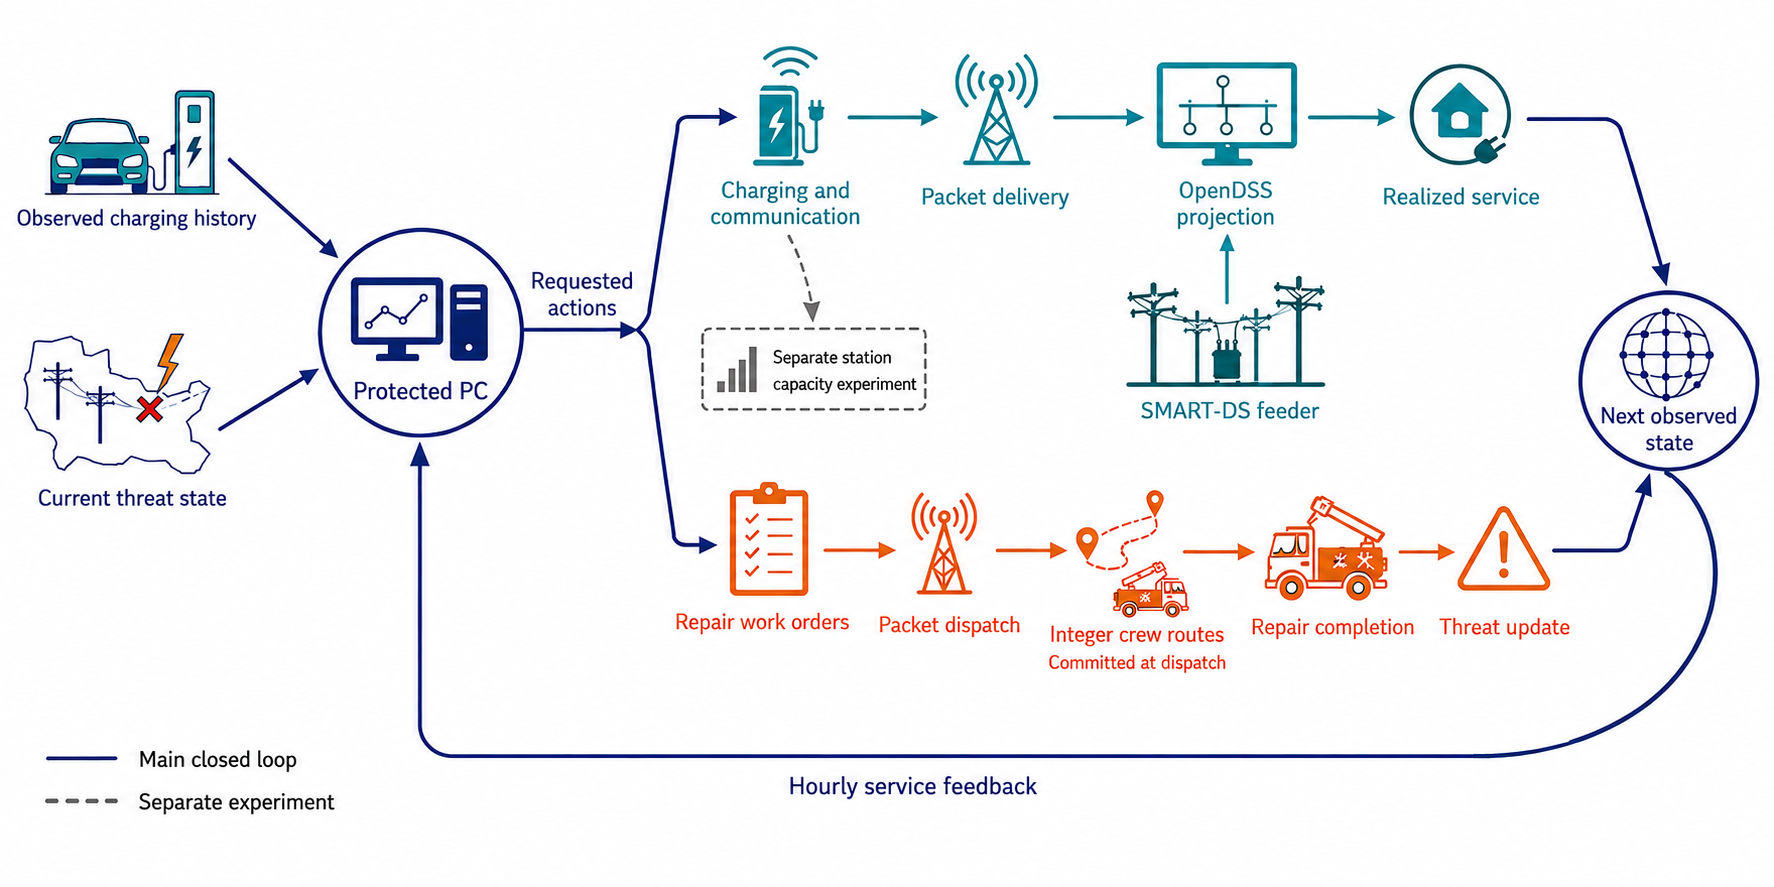
\includegraphics[width=\textwidth]{fig_executable_system.png}
\caption{Executable PC closed loop. Protected PC denotes PC with reference protection.
Observed charging history supplies the
shared forecast, and the controller receives the current scenario threat state.
EAGLE-I observations inform transition calibration and the repair duration prior.
Requested service actions pass through packet
delivery and SMART-DS/OpenDSS projection.  Repair work orders pass through
packet dispatch, integer routing, and recorded completion events.  Routes are
committed at dispatch, while service allocations are updated hourly.  Realized
service and threat updates form the next observed state.  The dashed path
denotes the separate station capacity experiment and is not part of the primary
4,096-scenario loop. The conceptual illustration was generated and edited with
OpenAI image tools, \protect\url{https://openai.com/}.}
\label{fig:executable-system}
\end{figure*}

\begin{table*}[t]
\centering
\caption{Independent evidence sources and their distinct roles}
\label{tab:evidence-sources}
\begin{tabular}{p{0.17\textwidth}p{0.18\textwidth}p{0.20\textwidth}p{0.35\textwidth}}
\toprule
Source & Scale & Observed fields & Role in this study \\
\midrule
City of Boulder EV sessions & 148,136 transactions from 50 stations between 2018 and 2023 & Arrival time, charging duration, energy (kWh), station and address & Measured charging demand with calendar periods for training, selection, and testing \\
EAGLE-I & 249,316,543 national rows with 819,528 retained in Boulder and six adjacent counties between 2014 and 2025 & County, UTC timestamp, customers out & Power state persistence, event and recovery distributions, and uncertainty bounds with missing rows preserved \\
SMART-DS SFO P1U feeder & 80 buses, 219 nodes, 27 loads, 67 lines, 13 transformers & OpenDSS circuit, equipment and peak load operating point & Online projection for all primary policy hours and the integrated electrical stress test \\
Packet and route models & 12,000 packet stress rows and 4,096 paired main scenarios with up to 36 jobs and four crews & Queue events, retries, deadlines, backup, integer crews, travel, service and completion times & Requested controls and threat updates after a recorded repair completion event \\
\bottomrule
\end{tabular}
\end{table*}


The primary demand source is the City of Boulder Electric Vehicle Charging
Station Data under a CC0 license.  Its metadata defines one
row as one transaction and provides local transaction time, station identity,
charging duration, and delivered energy.  The local archive contains all
148,136 transactions released from 2018 through 2023, with 50 station records and
1,252,719.654 measured positive kWh.  Four records lack an end time, 16,113
report zero energy, no duplicate source identifier or full row was found, and
no negative energy was retained.  Arrival counts are exact transaction counts
by start hour.  Session energy is measured.  Its hourly load profile is obtained
by spreading each session's energy uniformly over the reported
charging duration.  Conservation checks recover all 148,136 arrivals and the
measured positive energy to within 0.001 kWh.

Time was split before model fitting.  The period from 2018 through 2021 was used
for training, 2022 was used for model selection, and 2023 was used for final
testing.  No random row split crosses this
calendar boundary.  A second five fold spatial test withheld contiguous
west to east station blocks from target fitting.  In that inductive deployment
test, a held out station's calibration before 2022 and observed 1, 24, and 168 h
lags were permitted, but its target values never entered coefficient fitting.

Power event evidence came from the CC BY 4.0 EAGLE-I release
\cite{brelsford2024eaglei}.  The source record contained 17 files and
249,316,543 rows.  Preprocessing retained
819,528 observations for Boulder County and its six adjacent counties,
including 171,187 Boulder observations.  EAGLE-I timestamps are UTC and were
converted to America/Denver only for alignment with local charging records.
Because the source omits zero outage records and cannot distinguish a true zero
from a collection gap, absent county and time pairs were preserved as missing
rather than silently imputed as zero.  Events were evaluated at 50, 100, and
500 customers out.  At the 50-customer threshold, 2,535 events had median
duration 1.75 h and 90th percentile duration 6.5 h.  The post peak half recovery
time was observable for 19.6\% of events and had median 0.75 h.  These traces
inform a scenario distribution, not station level failure labels or utility
work orders.

The independent electrical test uses one complete SMART-DS v1.0 San Francisco
P1U feeder and its unmodified OpenDSS model.  The solved circuit contains 80
buses, 219 nodes, 27 loads,
67 lines, and 13 transformers.  Eighteen nodes already deenergized in the
released base case are identified and excluded from active voltage minima.
They are not counted as failures caused by EV action.  The base active node voltage
minimum is 0.989 p.u. and maximum line loading is 0.912 p.u.  Requested EV
actions are aggregated as balanced three phase, wye connected constant $PQ$
increments at the 17 eligible three phase loads.  Active power is the executed
station request and reactive power follows a 0.98 lagging power factor.  The
released load voltage level (0.48 or 12.47 kV) and base load parameters are
otherwise unchanged.  Twenty
station to load mappings are prepared in advance.  Mapping $s\bmod20$ is
shared by all policies in scenario $s$ and recorded in the scenario table.
At every simulated hour, station level executable charging is aggregated at the
assigned loads, OpenDSS solves the unprojected action, and a bisection backtracks
its common fraction until voltage lies in $[0.95,1.05]$ p.u., line loading is at
most 1.0 p.u., and the circuit converges.  Only this projected energy enters
served energy and backlog equations.  This gate validates the electrical
feasibility of a proposed charging action.  It does not simulate feeder
topology reconfiguration, switching or breaker operations, fault isolation,
feeder resupply, or equipment parameter changes after repair.  The experiment
therefore studies charging service restoration under a fixed feeder topology.

\subsection{Demand forecasting and spatial transfer}
\label{sec:forecast-results}

\begin{table}[t]
\centering
\caption{Calendar split test performance on measured Boulder charging sessions in 2023}
\label{tab:real-ev-forecast}
\begin{tabular}{lrrrr}
\toprule
Method & \multicolumn{2}{c}{Arrivals} & \multicolumn{2}{c}{Energy (kWh)} \\
 & MAE & RMSE & MAE & RMSE \\
\midrule
Historical mean & 0.137 & 0.517 & 1.101 & 3.026 \\
Weekly seasonal & 0.156 & 0.637 & 1.130 & 3.299 \\
Persistence & 0.175 & 0.678 & 1.059 & 3.186 \\
Graph recurrent forecaster & 0.110 & 0.527 & 0.945 & 3.113 \\
\bottomrule
\end{tabular}
\end{table}


Table~\ref{tab:real-ev-forecast} reports the fixed 2023 temporal test.  The
graph recurrent forecaster achieved arrival MAE 0.110 and energy MAE 0.948 kWh,
compared with 0.137 and 1.101 kWh for the historical mean.  Its energy RMSE
(3.119 kWh) did not beat the historical mean (3.026 kWh), so no uniform metric
dominance is claimed.  Across three training runs, arrival MAE ranged from 0.1097 to
0.1101 and energy MAE from 0.9449 to 0.9492 kWh.  The reported model was selected
by its validation score, not by the smallest test error among these runs.

The spatial test pooled all five held out blocks and six horizons.
The spatial ridge model reduced energy MAE from 1.130
to 1.054 kWh and RMSE from 2.928 to 2.272 kWh relative to station specific weekly
history.  Arrival RMSE also decreased from 0.557 to 0.440, but arrival MAE
(0.161) was worse than the pooled calendar mean (0.139).  Thus the measured data
forecast supports temporal deployment and improves several unseen station
endpoints.  Arrival MAE remains higher at sparse stations, which identifies the
forecast condition for interpreting the decision study.

\subsection{Propagation calibration and policy comparison}
\label{sec:policy-results}

\begin{table}[t]
\centering
\caption{Propagation coefficients and prespecified uncertainty set}
\label{tab:calibrated-uncertainty}
\begin{tabular}{lrrl}
\toprule
Parameter & Central & Interval & Evidence class \\
\midrule
$\rho_r$ & 0.728 & [0.546, 0.911] & estimated \\
$\sigma$ & 0.233 & [0.116, 0.349] & estimated \\
$\rho_p$ & 0.772 & [0.754, 0.787] & estimated \\
$\tau_{pr}$ & 0.000 & [0.000, 0.032] & estimated observational \\
$\tau_{pc}$ & 0.427 & [0.169, 0.551] & constructed \\
$\rho_c$ & 0.500 & [0.300, 0.800] & sensitivity only \\
$\tau_{rc}$ & 0.040 & [0.000, 0.080] & sensitivity only \\
$\tau_{cr}$ & 0.080 & [0.000, 0.160] & sensitivity only \\
$\tau_{cp}$ & 0.040 & [0.000, 0.080] & sensitivity only \\
\bottomrule
\end{tabular}
\end{table}


The coefficient ledger in Table~\ref{tab:calibrated-uncertainty} distinguishes
estimated, observational, constructed, and sensitivity range quantities.  A
nonnegative station deficit regression estimated mobility persistence and
spatial spread from 1,268,661 training samples.  A separate county level
regression checks the aligned outage and charging series.  On 3,108 aligned
2023 test hours, that regression's road state RMSE was 0.306 versus 0.374 for
persistence.  It is not the station propagation model used to construct $M$.
EAGLE-I estimated power persistence at 0.772 with a 90\% day block bootstrap interval
$[0.754,0.787]$.  The aligned coefficient from power state to EV deficit was effectively
zero with upper interval 0.032, providing no evidence for a strong direct
conditional association.  The packet model constructed the
power to communication interval from 12,000 training period packet scenarios.
Its fitted central coefficient is 0.427 and its hour block bootstrap interval
is $[0.169,0.551]$.  Directions without joint field traces span
sign constrained sensitivity ranges including zero.

Central PC scores each route using the continuous service objective in
\eqref{eq:route-service-score} under the calibrated transition.  Forecast
matched uses the same objective, demand forecast, backlog update, completion
schedule, and route candidates, but holds unrepaired threats at their current
values.  Robust PC instead minimizes the largest predicted service cost over
21 declared matrices.  The two exposure score controls retain the earlier
route ranking rules, one based on current exposure and one on propagated
exposure.  This comparison separates the contribution of service cost scoring
from the additional effect of propagation.  All five selectors share the same
candidate set, including candidates constructed from central and worst set
priorities.  Only their final scoring rule changes.  Static and greedy use
their own direct route priorities, and the oracle alone receives future demand
and innovations.  These eight policies isolate service scoring and propagation.
Table~\ref{tab:policy-definitions} also defines PC with reference protection,
which changes the route acceptance rule while keeping the same execution
conditions.  The mechanism comparisons below retain their original controls
and statistical families.

The service score was compared with exposure scoring on 512 validation
scenarios from 2022 before the revised test.  Central service scoring reduced
cost by 8.707 relative to exposure matched, with a paired interval
$[-11.113,-6.466]$.  Its difference from the same service score without
propagation was $-0.095$ with interval $[-0.950,0.754]$.  The score definition,
weights, budgets, and forecast selection rule were then fixed for the test,
which retained both exposure controls and the stronger service matched control.
Normalization and budgets use only 2018 through 2021 station statistics.
Forecast selection uses 2022 error, and every target window lies entirely
within its declared calendar period.
Earlier revision checks had examined results from the same test year.
The present comparisons evaluate the subsequently fixed specification on that year.

The test comprised 4,096 paired scenarios with 1,024 per threat class.
Realized coefficients were drawn independently from their stated ranges for
each scenario and were shared across policies.  The primary comparison family
contains central PC versus each of the three service and exposure controls,
both overall and in the four classes.  We report paired bootstrap intervals
with 20,000 resamples, paired $t$ tests, and two sided Wilcoxon tests.  Holm
correction includes all fifteen comparisons separately for each test.
Bootstrap intervals are marginal intervals, not simultaneous intervals for the
whole family.  Table~\ref{tab:supp-primary} retains every comparison.
The Appendix, part~\ref{app:parameters}, reports each value, unit, role, calibration rule,
selection source, and tested range in
Tables~\ref{tab:scenario-parameters}, \ref{tab:complete-parameters}, and
\ref{tab:execution-parameters}.

\begin{table*}[t]
\centering
\caption{Policy information and execution contract.  ``Current'' means the
observation available at the decision hour.  The common route portfolio contains
routes induced by static, greedy, forecast-matched, central-PC, robust-PC, and
uniform priorities.  Future innovations are never revealed to deployable
policies.}
\label{tab:policy-definitions}
\scriptsize
\setlength{\tabcolsep}{2.4pt}
\begin{tabular}{p{0.10\textwidth}p{0.10\textwidth}p{0.10\textwidth}p{0.09\textwidth}p{0.125\textwidth}p{0.085\textwidth}p{0.155\textwidth}p{0.125\textwidth}}
\toprule
Policy & Demand information & Threat/backlog & Multi-step transition rollout & Transition matrix used & Future innovations & Repair-route rule & Common execution gates \\
\midrule
Static & Historical station mean & Backlog only for charging & No & None & No & Direct route from static priority & Yes \\
Greedy & Common forecast & Current threat and backlog & No & None & No & Direct route from current-threat priority & Yes \\
Forecast-matched & Common forecast & Current threat and backlog & No & None & No & Current-exposure score over common portfolio & Yes \\
Central PC & Common forecast & Current threat and backlog & Yes & Calibrated central $M$ & No & Central-transition score over common portfolio & Yes \\
Robust PC (extension) & Common forecast & Current threat and backlog & Yes & Worst score over 21 declared matrices & No & Worst-transition score over common portfolio & Yes \\
Oracle & Realized future demand & Current threat and backlog & Yes & Central $M$ & Yes & Direct route from oracle priority & Yes \\
\bottomrule
\end{tabular}
\end{table*}


\begin{table}[t]
\centering
\caption{Central PC compared with the same service score without threat propagation, followed by all policy means. Positive reduction denotes lower cost than forecast matched. $\Delta$ is central minus matched cost. Intervals are paired marginal intervals. All policies share 4,096 scenarios and the oracle alone observes future demand and innovations.}
\label{tab:robust-boulder}
\footnotesize
\setlength{\tabcolsep}{3pt}
\resizebox{\columnwidth}{!}{%
\begin{tabular}{@{}lrrrr@{}}
\toprule
Group & Pairs & Reduction (\%) & $\Delta$ & $\Delta$ 95\% CI \\
\midrule
All & 4096 & 0.1027 & -1.1436 & [-1.5257, -0.7704] \\
Nominal & 1024 & -0.0002 & 0.0013 & [-0.0042, 0.0075] \\
Single domain & 1024 & 0.0132 & -0.1021 & [-0.2602, 0.0510] \\
Cascade & 1024 & 0.0741 & -0.7946 & [-1.7624, 0.1327] \\
OOD compound & 1024 & 0.1979 & -3.6789 & [-4.8554, -2.5890] \\
\bottomrule
\end{tabular}
}
\vspace{3pt}
\begin{tabular}{@{}lrr@{}}
\toprule
Policy & Mean cost & Reduction (\%) \\
\midrule
Forecast matched & 1113.68 & 0.0000 \\
Central PC & 1112.54 & 0.1027 \\
Robust PC & 1112.90 & 0.0697 \\
Exposure matched & 1120.23 & -0.5885 \\
Exposure central & 1124.63 & -0.9832 \\
Static & 1202.74 & -7.9970 \\
Greedy & 1122.54 & -0.7960 \\
Oracle & 1053.67 & 5.3887 \\
\bottomrule
\end{tabular}
\end{table}


Table~\ref{tab:robust-boulder} reports the primary paired comparison and the
policy summary.  Central PC reduced mean cost by 0.1027\% relative to the same
service score without propagation.  The paired difference was $-1.1436$ with
95\% interval $[-1.5257,-0.7704]$, and the Holm adjusted paired $t$ and Wilcoxon
probabilities were $1.38\times10^{-8}$ and $9.79\times10^{-23}$.  The OOD
compound class showed a 0.1979\% reduction with difference interval
$[-4.8554,-2.5890]$.  The nominal, single domain, and cascade mean intervals
included zero.  Their reductions were $-0.0002\%$, 0.0132\%, and 0.0741\%,
respectively.  Thus the overall effect is statistically distinguishable but
small, and a uniform classwise improvement is not established.  These intervals
quantify Monte Carlo scenario uncertainty conditional on the public data and
simulation model rather than variation across utilities.

The larger effect came from evaluating service rather than exposure alone.
Central PC reduced mean cost by 0.6872\% relative to exposure matched and
1.0753\% relative to exposure central, with difference intervals
$[-8.3843,-7.0077]$ and $[-13.1616,-11.0704]$.  Both overall comparisons remained
significant after Holm correction.  The service matched control also had lower
mean cost than either exposure control.  These results locate most of the gain
in the route objective, with a smaller additional contribution from propagation.
The oracle mean was 1053.67 compared with 1112.54 for central PC, leaving a
5.59\% policy to oracle gap.  This is an information reference, not a bound on
the globally optimal restoration schedule.

Robust PC had mean cost 1112.90.  Its difference from central PC was 0.3670,
with marginal interval $[0.0788,0.6627]$.  Its upper 5\% and 1\% conditional
mean costs exceeded central PC by 2.85 and 4.73, respectively, while the maximum
observed cost was identical at 4494.26.  The conditional means include a
fractional observation at the empirical quantile boundary.  These descriptive
tail comparisons do not establish a tail protection benefit, and the worst set
calculation remains a sensitivity extension rather than the principal method.
Table~\ref{tab:supp-cost-tail} reports the empirical cost tails of the eight mechanism controls.

\begin{table}[t]
\centering
\caption{Objective sensitivity of central PC relative to forecast matched. All rows use the same 1,024 scenario inputs. Candidate routes are selected again under each stated objective. Reference is the corresponding subset of the primary experiment, not its full 4,096 pairs.}
\label{tab:objective-sensitivity}
\footnotesize
\setlength{\tabcolsep}{3pt}
\resizebox{\columnwidth}{!}{%
\begin{tabular}{@{}lrr@{}}
\toprule
Weights & Reduction (\%) & Difference (95\% CI) \\
\midrule
Reference & 0.0995 & -1.1299 [-1.9426, -0.3834] \\
$2\times$ mobility & 0.1028 & -1.1782 [-2.0284, -0.3950] \\
$2\times$ unserved energy & 0.0597 & -1.1458 [-2.0653, -0.3006] \\
$2\times$ communication & 0.1029 & -1.3283 [-2.3910, -0.3448] \\
$2\times$ power service & 0.1264 & -1.4710 [-2.5631, -0.4754] \\
$0.5\times$ cascade & 0.0810 & -0.8553 [-1.5909, -0.1857] \\
\bottomrule
\end{tabular}
}
\end{table}


Table~\ref{tab:objective-sensitivity} changes one objective weight at a time
and reruns candidate selection and execution on the same 1,024 scenario inputs.
The reference row is the corresponding subset of the primary experiment.
Across the five changed objectives, central PC reductions ranged from 0.0597\%
to 0.1264\%, with marginal mean difference intervals below zero.  The direction
of the comparison therefore persisted under these weight changes.  However,
none of their paired mean tests remained significant after correction across
the full 45 comparison sensitivity family.  These results describe dependence
on the service objective without claiming uniform statistical evidence across
all objectives.  Table~\ref{tab:supp-sensitivity} reports the adjusted probabilities.

\begin{figure*}[t]
\centering
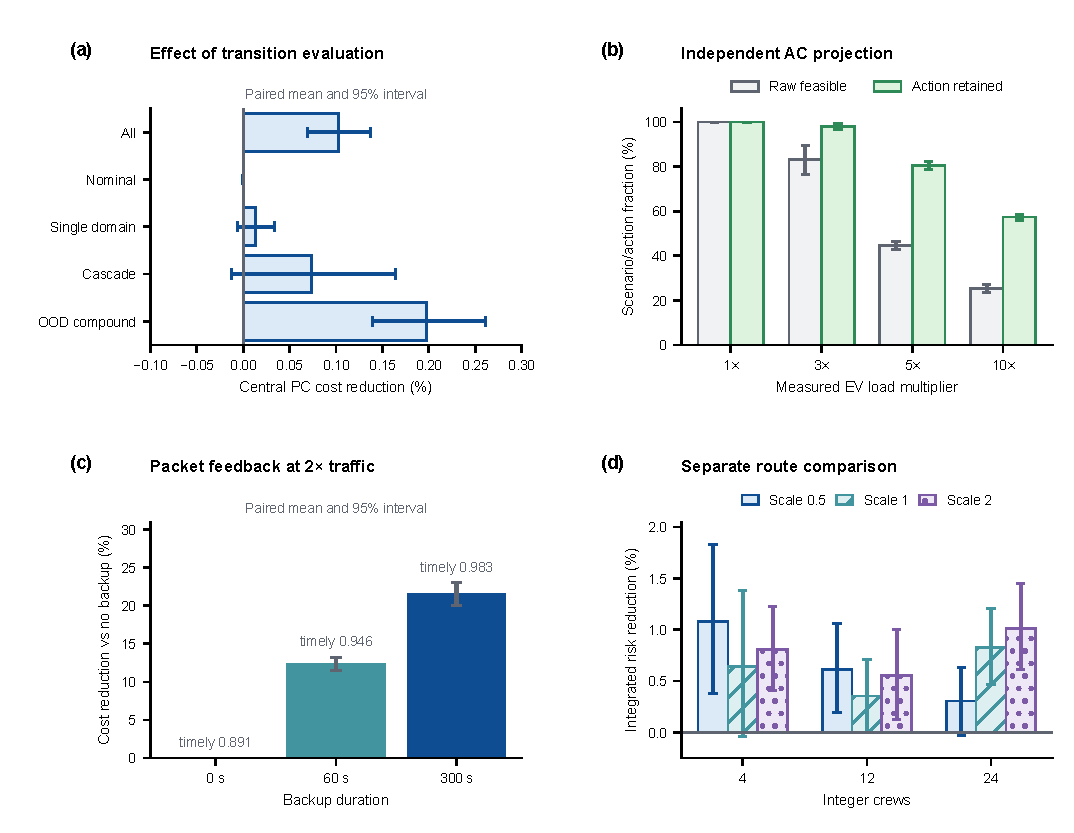
\includegraphics[width=\textwidth]{fig_operational_evidence.pdf}
\caption{Decision and execution evidence.  Panel (a) reports the central PC cost
reduction relative to the forecast matched baseline.  Filled intervals show
paired means and bootstrap confidence limits for each threat class and for all
scenarios.  Panel (b) reports raw distribution system feasibility and the
fraction of requested EV action retained after projection, with normal
approximation intervals across 20 mappings of 24 hours each.  Panel (c) reports
the cost reduction from backup power under increased packet traffic, with the
mean fraction of actions delivered on time printed above each bar.  Panel (d)
reports the separate integrated risk comparison when executable routes are
evaluated before selection.  Panels (a), (c), and (d) show paired bootstrap
95\% intervals, using 4,096 pairs overall and 1,024 per class in (a), 1,024 in
(c), and 128 per crew and service condition in (d).  Paired $t$ and Wilcoxon
tests with their stated Holm families are reported in the tables.  Percentage
intervals divide the cost or risk difference interval by the observed reference
mean.}
\label{fig:operational-evidence}
\end{figure*}

Figure~\ref{fig:operational-evidence} places the primary transition comparison
beside the electrical, communication, and crew execution results.  The panels
use the same values and sample definitions as the corresponding tables.

\subsection{Electrical and mobility execution}
\label{sec:grid-results}

\begin{table}[t]
\centering
\caption{Electrical projection and repair completion in the integrated experiments. Primary includes eight policies and stress includes six. Action retention is the mean hourly fraction. Job completion is the mean scenario fraction of requested jobs completed within the horizon.}
\label{tab:integrated-execution}
\footnotesize
\setlength{\tabcolsep}{3pt}
\resizebox{\columnwidth}{!}{%
\begin{tabular}{@{}lrrrr@{}}
\toprule
Condition & Pairs & AC hours & Raw infeas. & After proj. \\
\midrule
Measured load & 4,096 & 196,608 & 0 & 0 \\
$20\times$ EV load & 1,024 & 36,864 & 348 & 0 \\
\bottomrule
\end{tabular}
}
\vspace{3pt}
\begin{tabular}{@{}lrr@{}}
\toprule
Condition & Action retained (\%) & Jobs completed (\%) \\
\midrule
Measured load & 100.00 & 81.05 \\
$20\times$ EV load & 99.80 & 81.12 \\
\bottomrule
\end{tabular}
\end{table}


Table~\ref{tab:integrated-execution} summarizes the feeder and crew outcomes in
the main loop.  The primary run with 4,096 scenarios made 196,608 online OpenDSS calls, one for each
scenario, policy, and hour.  At measured load, all raw actions were already feasible,
so projection retained 100\% of requested charging.  This feasibility
result does not by itself demonstrate feedback.  The companion $20\times$
stress run therefore scaled both new energy demand and the charging budget,
using 1,024 paired scenarios and six policies in the same loop.  It produced
348 infeasible policy hours.  Projection reduced this count to zero,
retained 99.80\% of requested service on average, and placed 16,660.6 kWh of
curtailed energy into unserved demand/backlog rather than crediting it as served.
Thus the online adapter changes downstream state whenever the AC limit binds.

\begin{table}[t]
\centering
\caption{SMART-DS AC action projection (20 mappings, 24 hours each)}
\label{tab:smartds-action-loop}
\resizebox{\columnwidth}{!}{%
\begin{tabular}{lrrrr}
\toprule
EV load & Raw feasible (\%) & Action retained (\%) & Raw $V_{\min}$ & Raw line p.u. \\
\midrule
1$\times$ & 100.0 & 100.0 & 0.986 & 0.929 \\
3$\times$ & 83.1 & 98.0 & 0.977 & 0.968 \\
5$\times$ & 44.6 & 80.5 & 0.966 & 1.044 \\
10$\times$ & 25.4 & 57.3 & 0.938 & 1.361 \\
\bottomrule
\end{tabular}
}
\end{table}


Table~\ref{tab:smartds-action-loop} extends the electrical comparison across
load multipliers.  The SMART-DS experiment comprised 20 randomized station to load mappings, 24
test hours, and four EV load multipliers (1,920 cases).  Raw actions were all
feasible at measured load.  At $3\times$, $5\times$, and $10\times$ load, raw
feasibility fell to 83.1\%, 44.6\%, and 25.4\%, whereas the action projection
retained 98.0\%, 80.5\%, and 57.3\% of requested EV power.  Every projected
case converged and met the voltage and line limits.  A separate test for all of 2023
used all 7,451 nonzero hours at $1\times$ and $3\times$ load (14,902 cases).
At $3\times$, 99.17\% of raw actions were feasible and projection retained
99.94\% on average.  All projected cases remained feasible.  The reported
curtailment is therefore produced inside the action path and not inferred from
a later voltage label.

\begin{table}[t]
\centering
\caption{Station choice under measured demand for 24 peak hours}
\label{tab:station-choice}
\resizebox{\columnwidth}{!}{%
\begin{tabular}{rrrrrr}
\toprule
Closure (\%) & No choice & Nearest & Logit & Coordinated & Extra km \\
\midrule
10 & 67.4 & 100.0 & 100.0 & 100.0 & 0.32 \\
20 & 55.8 & 100.0 & 100.0 & 100.0 & 0.50 \\
30 & 43.7 & 100.0 & 100.0 & 100.0 & 0.97 \\
\bottomrule
\end{tabular}
}
\end{table}


Table~\ref{tab:station-choice} reports the station reassignment results.  Station
closure does not automatically imply abandoned charging.  A separate
capacity constrained flow model distinguished local service, rerouting, and
unserved demand across 24 observed peak hours.  Under measured demand and 10,
20, and 30\% closures, preserving the original station served only 67.4, 55.8,
and 43.7\% of energy.  Nearest, logit, and coordinated reassignment all served
100\% in these cases.  The coordinated solution required only 0.32, 0.50, and
0.97 km energy weighted extra distance.  Under $4\times$ demand, total
constructed capacity, rather than the choice model, became the limiting factor.
This stress result prevents the rerouting mechanism from creating fictitious
capacity.

\subsection{Communication and crew execution}
\label{sec:crew-results}

The packet emulator is a finite buffer queue with first come, first served
discipline, discrete events, erasures, two retransmissions, backoff, a 500 ms control deadline,
and explicit backup duration.  An M/M/1 unit test at 10 packet/s arrival and
20 packet/s service reproduced the theoretical 100 ms mean latency with 0.269\%
relative error.  Across 12,000 station stress cases, the original algebraic
support proxy had Spearman correlation 0.860 but mean absolute error 0.243
against the simulated fraction of actions delivered on time, which confirms that the proxy
cannot replace packet dynamics.

\begin{table}[t]
\centering
\caption{Backup duration for central PC at $2\times$ packet traffic on 1,024 paired scenarios. Completion is the fraction of requested jobs completed. Cost differences compare the same policy with no backup.}
\label{tab:packet-feedback}
\footnotesize
\setlength{\tabcolsep}{3pt}
\resizebox{\columnwidth}{!}{%
\begin{tabular}{@{}lrrrr@{}}
\toprule
Backup & Timely action & Completion & Reduction (\%) & Difference 95\% CI \\
\midrule
0 s & 0.891 & 0.754 & 0.00 & Reference \\
60 s & 0.946 & 0.790 & 12.35 & [-186.05, -161.06] \\
300 s & 0.983 & 0.819 & 21.55 & [-323.85, -281.66] \\
\bottomrule
\end{tabular}
}
\end{table}


Table~\ref{tab:packet-feedback} reports the effect of backup duration.
Equation~\eqref{eq:packet-derate} closes this evidence loop.  Under prespecified
$2\times$ traffic and 1,024 paired uncertain transition scenarios, 60 s backup
raised the mean timely action fraction to 0.946 and reduced central PC cost
by 12.35\% relative to no backup (difference CI $[-186.0,-161.1]$).  A 300 s
backup raised the fraction to 0.983 and reduced cost by 21.55\% (difference CI
$[-323.8,-281.7]$).  Both paired mean tests remained significant after Holm
correction across the two backup comparisons.  Before backup exhaustion, power threat caused no direct
service rate derating.  The effect arose only after the coded depletion event.

\begin{table}[t]
\centering
\caption{Route evaluated PC compared with matched routing}
\label{tab:route-crew}
\resizebox{\columnwidth}{!}{%
\begin{tabular}{rrrrr}
\toprule
Crews & Service scale & Risk reduction (\%) & Difference 95\% CI & Holm $p$ \\
\midrule
4 & 0.5 & 1.08 & [-2.25, -0.47] & 0.0237 \\
4 & 1.0 & 0.64 & [-2.33, 0.06] & 0.177 \\
4 & 2.0 & 0.81 & [-2.85, -0.94] & 0.00175 \\
12 & 0.5 & 0.61 & [-0.65, -0.12] & 0.0492 \\
12 & 1.0 & 0.35 & [-0.68, 0.00] & 0.129 \\
12 & 2.0 & 0.55 & [-1.63, -0.20] & 0.00652 \\
24 & 0.5 & 0.31 & [-0.30, 0.01] & 0.0293 \\
24 & 1.0 & 0.83 & [-0.94, -0.37] & 6.49e-05 \\
24 & 2.0 & 1.01 & [-1.95, -0.82] & 6.91e-06 \\
\bottomrule
\end{tabular}
}
\end{table}


In the integrated primary run, the route generated for four crews was not a diagnostic added
after scoring.  The same work order set was dispatched through packet delivery,
and threat was updated only at its recorded completion hours.  Central PC
completed a mean 81.20\% of requested jobs within the horizon versus 81.10\%
for forecast matched.  The fraction is calculated separately in each scenario
before averaging, and its denominator includes requests not dispatched.
The paired difference interval was $[0.00058,0.00147]$.  Mean scheduled
completion time among dispatched jobs fell from 3.119 to 3.097 h, with
difference interval $[-0.02643,-0.01802]$ h.  This time includes jobs whose
scheduled completion extends beyond the service horizon.  Total scheduled
travel was 2.621 versus 2.619 h per scenario, with difference interval
$[-0.00358,0.00765]$ h.  The completion fraction and time comparisons remained
significant after correction across nine secondary service and physical
endpoints, whereas travel did not improve detectably.
Table~\ref{tab:supp-physical} reports all nine outcomes.  Unserved energy decreased
by 0.0369 kWh per scenario, while electrical loss increased by
$1.53\times10^{-6}$ MWh, with interval
$[0.60,2.46]\times10^{-6}$ MWh.  Both electrical changes were small.  The voltage and
timely action mean intervals included zero, and neither action retention nor
curtailment differed at measured load.
Loss and voltage measurements used separate OpenDSS contexts at convergence
tolerance $10^{-10}$, compared with $10^{-8}$, and at most 100 iterations.
The contexts received identical accepted loads for all 4,096 central and matched
pairs without changing scores, routes, executed service, or the original
$10^{-4}$ execution tolerance.  The largest scenario differences between
measurement tolerances were $9.94\times10^{-8}$ MWh and
$6.35\times10^{-10}$ p.u., respectively.

Table~\ref{tab:route-crew} reports the route comparison for every crew and
service condition.  The route experiment used 36 jobs, integer fleets of 4, 12, and 24 crews,
geocoded travel at 30 km/h with 1.25 circuity, and service time multipliers
0.5, 1, and 2.  Each repair completion causally removed that job's risk from
the accumulated state.  The original PC priority lost its advantage in some
integer routed cases.  Route evaluated PC corrected this result by selecting the
lowest predicted risk executable candidate rather than projecting a continuous
priority after the decision.  In 128 independent scenarios per cell,
route evaluated PC reduced mean integrated risk in all nine crew and service
conditions by 0.31\% through 1.08\%.  Six bootstrap intervals excluded zero and seven
Holm adjusted Wilcoxon tests were below 0.05.  The intervals for four crews at
scale 1.0, twelve crews at scale 1.0, and twenty four crews at scale 0.5 included
zero and remain visible in
Table~\ref{tab:route-crew}.  The observed gain is not declared
uniformly significant.  The Holm adjusted Wilcoxon value for twenty four crews
at scale 0.5 is below
0.05 while its bootstrap interval crosses zero because the two procedures test
different statistics.  The interval targets the paired mean difference, whereas
Wilcoxon ranks the nonzero paired differences and is affected differently by
ties and skewness.  We therefore require the mean interval, not either test in
isolation, for a mean improvement claim.

The integrated sensitivity study holds the realized coefficient distribution
fixed while perturbing the matrix available to the controller.  Each condition
uses the same 1,024 scenario inputs.  With $0.75M$, central PC exceeded matched
cost by 3.7779, with marginal interval $[2.4720,5.0919]$, whereas robust PC was
3.6909 below central PC with interval $[-4.7773,-2.6813]$.  With $1.25M$, central
PC reduced matched cost by 1.2737, with interval $[-2.0959,-0.5635]$.  Under
coefficient noise of 0.15, the difference was $-1.8341$ with interval
$[-2.6349,-1.1321]$.  Robust PC exceeded central PC by 3.4569 and 1.2651 in
these latter conditions.  Thus worst set scoring offset the underscaled
transition in one condition but did not provide uniform protection.  The
calibrated transition's primary advantage also did not persist under every
matrix error.  Table~\ref{tab:supp-sensitivity} gives these comparisons with the full
sensitivity family and its multiplicity correction.

To distinguish uncertainty in the controller from uncertainty in the realized
environment, additional runs changed only the realized coefficients.  The
communication persistence and four couplings without joint field estimates
were set to zero individually and together, or doubled together, while the
controller retained its calibrated matrix and declared uncertainty set.
Setting all five quantities to zero gave a central minus matched difference
of $-1.1745$, with marginal interval $[-1.7176,-0.6815]$, a 0.1156\% reduction.
The individual zero settings also had negative mean differences, although
this alone does not establish significance across the full comparison family.
Doubling the five quantities gave $0.2837$ with interval $[-0.7188,1.2761]$,
so a mean benefit was not established in that condition.  Robust PC was then
2.0608 below central PC, with interval $[-2.9543,-1.2204]$.

A separate test changed the form of the realized transition rather than its
linear coefficients alone.  With $\mathsf A_{\rm sp}=\mathrm{diag}(A,A,A)$, the
propagated state before innovations and completion was
\begin{equation}
T(\zeta)=0.98\left[\mathbf1-\exp\left(
-\frac{[M_{\rm real}\zeta]_+ +0.15(\mathsf A_{\rm sp}\zeta)^{\odot2}}{0.98}
\right)\right],
\label{eq:nonlinear-test}
\end{equation}
where the exponential and square act componentwise.  Execution then used
$D(\bar r_h)\Pi_{\mathcal Z}(T(\zeta_h)+\xi_h)$.
The quadratic spatial term and saturation in \eqref{eq:nonlinear-test} are
absent from the controller's linear matrix family.  On 1,024 paired scenarios,
central PC reduced matched cost by 0.1532\%, with difference $-1.5148$ and
interval $[-1.9601,-1.1040]$.  Robust PC exceeded central PC by 0.7813, with
interval $[0.4315,1.1492]$.  These results test a distinct transition form
without changing the scoring rule or granting future information to the policy.
Table~\ref{tab:supp-sensitivity} retains every zero coupling, expanded coupling, and
nonlinear comparison alongside the matrix error tests.

\subsection{Reference protection and independent charging input}
\label{sec:reference-protection}

The matrix error comparisons motivate protection relative to a common
executable route.  We fixed the rule in \eqref{eq:protected-route} before
running its validation and evaluation.  Validation used 512 paired 2022
scenarios in each of seven conditions and compared
$\nu\in\{0,0.00025,0.0005,0.001\}$.  A candidate margin first had to limit
its original-condition mean cost increase over central PC to 0.05\% of
matched cost.  Among passing margins, selection minimized mean positive
excess above matched across the six perturbed conditions, with ties assigned
to the smaller margin.  Both route portfolios selected $\nu=0.001$.
Table~\ref{tab:guarded-validation} retains all validation choices.
The subsequent 2023 evaluation used 4,096 original-condition pairs and
1,024 pairs in each of the six perturbed conditions and electrical stress.
Because this year had already been examined during revision, it was a
fixed-rule reevaluation rather than an unused test year.

Let $E^+(P)=n^{-1}\sum_i[Q_i(P)-Q_i(P_b)]_+$, where each $P_b$ is the
matched route for that scenario and portfolio.  This quantity measures
additional cost incurred when a method performs worse than its reference.
It differs from the upper tail of total cost, which also includes scenario
severity shared by every policy.  For the aggregate error comparison, we
first averaged the six condition-specific positive-excess differences
within each of the 1,024 scenario identifiers.  Resampling those identifiers
preserved dependence between the conditions.  Mean intervals used 20,000
paired resamples.  The two portfolio comparisons received Holm adjustment,
while all 80 additional mean-cost comparisons formed a separate family.
The original-condition noninferiority check required a one-sided 97.5\%
bootstrap upper bound below zero for
$Q_i(P_g)-Q_i(P_c)-0.0005Q_i(P_b)$.

\begin{table}[t]
\centering
\caption{Reference protection on the original common routes. $G$ denotes PC with reference protection and $C$ central PC. $E^+$ is the mean positive excess cost above forecast matched. Intervals are paired marginal 95\% intervals. The original condition has 4,096 pairs and each other condition has 1,024 pairs.}
\label{tab:guarded-primary}
\footnotesize\setlength{\tabcolsep}{3pt}\renewcommand{\arraystretch}{1.12}
\begin{tabular}{@{}p{.22\columnwidth}p{.40\columnwidth}rr@{}}
\toprule
Condition & $G-C$ [95\% CI] & $E_C^+$ & $E_G^+$ \\
\midrule
Original & 0.0375 [-0.2279, 0.3017] & 1.0834 & 0.0657 \\
$0.75M$ & -3.0865 [-4.1245, -2.1035] & 5.5237 & 2.0125 \\
$1.25M$ & 0.6297 [0.0687, 1.2777] & 0.6728 & 0.0689 \\
Noise 0.15 & 0.9903 [0.5097, 1.5282] & 0.2862 & 0.0450 \\
Couplings doubled & -1.2044 [-2.0505, -0.3899] & 2.5848 & 0.1524 \\
Couplings zero & 0.4804 [0.1196, 0.8722] & 0.4702 & 0.0197 \\
Nonlinear & 0.7658 [0.4804, 1.0707] & 0.2579 & 0.0088 \\
Electrical stress & -0.6917 [-5.9540, 4.6563] & 10.7569 & 1.3159 \\
\bottomrule
\end{tabular}
\end{table}


On the original routes, reference protection retained a mean cost of
1112.5728, compared with 1112.5353 for central PC and 1113.6789 for matched.
The protected minus matched difference was $-1.1061$, with interval
$[-1.3760,-0.8582]$ and Holm adjusted paired $t$ probability
$3.93\times10^{-15}$.  The reduction was 0.0993\%.  Its mean penalty relative
to central PC was 0.0375, or 0.0034\%, and the noninferiority upper bound
was $-0.2550$.  The rule accepted a replacement in 6.20\% of scenarios.
Consequently, most routes remained matched, but the replacements retained
most of central PC's average benefit.  The fraction of scenarios worse than
matched fell from 11.94\% for central PC to 0.90\%, and $E^+$ fell from
1.0834 to 0.0657.  These frequencies describe realized outcomes rather than
an unconditional guarantee from the model score.

Across the six error conditions, the paired decrease in positive excess was
1.2481, with interval $[-1.4785,-1.0296]$ for protected minus central and
Holm adjusted probability $6.80\times10^{-26}$.
Table~\ref{tab:guarded-primary} shows the individual conditions as well.
Protection reduced additional losses under an underscaled matrix and
expanded unobserved couplings, but it gave up some of central PC's average
gain under an enlarged matrix, coefficient noise, zero couplings, and
nonlinear propagation.  Positive-excess protection is therefore a selective
tradeoff, not uniform mean superiority.  Nor does it imply lower total-cost
tails.  The original-condition upper 5\% mean cost exceeded central PC by
2.7673, with exploratory interval $[0.3615,5.5575]$.  Both portfolio tail
comparisons are retained in Table~\ref{tab:guarded-tails}.

The separate parameter-independent route construction tests whether a
favorable score ablation could arise from using unknown parameters to
generate the routes.  Table~\ref{tab:guarded-ablation} reports all conditions
on this common alternative portfolio.  Removing the five unsupported terms
from the score increased original-condition cost over central PC by 0.9937,
with interval $[0.7761,1.2289]$ and Holm adjusted probability
$1.26\times10^{-15}$.  Thus simply deleting those terms did not resolve
parameter uncertainty.  Reference protection instead increased mean cost by
0.1039 while passing the fixed noninferiority check, whose upper bound was
$-0.3419$.  Its aggregate positive-excess decrease was 0.1823, with interval
$[-0.2691,-0.1089]$ and Holm adjusted probability $1.01\times10^{-5}$.
Its mean benefit over matched did not survive the full comparison correction.
These results support the protection mechanism on a second route construction
without attributing differences between the portfolios to a single score.

An independent geographic input used the City of Palo Alto charging
records.\footnote{City of Palo Alto, Electric Vehicle Charging Station Usage,
published February 2021. The source record is available at
\url{https://data.paloalto.gov/dataviews/257812/electric-vehicle-charging-station-usage-july-2011-dec-2020/}.}
The complete municipal source contained 259,415 sessions.  Fixed quality
rules and a requirement of at least 100 valid sessions in 2017 and 2018
retained 33 stations and 159,587 sessions during 2017 to 2020, including
20,042 in the 2020 evaluation year.  Arrival counts and session energy were
observed.  Hourly energy was reconstructed uniformly over the reported
charging duration, giving 1,416,780.194 kWh and conserving retained energy
to numerical precision.  Station eligibility, coordinates, mean demand,
and budgets used 2017 and 2018 only.  The charging, communication, and
repair priority budgets were 54.4678 kWh per hour, 50.3244 service units,
and 10 priority units, with the same construction rules as Boulder.

The restoration parameters and selected margin were unchanged.  One demand
input used the selected Boulder graph model with identical learned weights
and normalization, replacing only the nonlearned adjacency by the Palo Alto
station graph.  This was a retrospective geographic transfer, not a claim
that the later-trained model had been deployed in 2020.  The second input
used the corresponding hours of the preceding week.  Both forecasts were
fixed before computing external policy outcomes and were evaluated separately.
The electrical feeder, abstract transition, communication conditions, and
repair duration model were retained, while route distances used the new
station coordinates.  Constructed packet response functions were assigned
by station index.  The new observations therefore test charging demand and
station geometry rather than a jointly observed local infrastructure event.

\begin{table}[t]
\centering
\caption{Independent municipal charging input with 1,024 pairs per row. Original and independent identify the two common route portfolios. Reduction is relative to forecast matched. The final column is the one-sided 97.5\% upper bound after subtracting the fixed 0.05\% noninferiority margin.}
\label{tab:guarded-transfer}
\footnotesize\setlength{\tabcolsep}{3pt}\renewcommand{\arraystretch}{1.12}
\begin{tabular}{@{}p{.24\columnwidth}p{.38\columnwidth}rr@{}}
\toprule
Forecast and routes & $G-C$ [95\% CI] & Red. (\%) & NI upper \\
\midrule
Graph, original & -0.2826 [-0.6408, 0.0433] & 0.1806 & -0.2173 \\
Graph, independent & -0.0227 [-0.1109, 0.0607] & 0.0124 & -0.1828 \\
Weekly, original & -0.1761 [-0.4869, 0.1121] & 0.1338 & -0.1487 \\
Weekly, independent & -0.0735 [-0.1912, 0.0278] & 0.0169 & -0.2193 \\
\bottomrule
\end{tabular}
\end{table}


Each input used 1,024 paired scenarios per condition, with all eight
conditions and both portfolios retained.  External mean comparisons formed
one 160-test Holm family.  On the original routes, reference protection
reduced matched cost by 0.1806\% with the graph forecast and 0.1338\% with
weekly persistence, with adjusted probabilities 0.00481 and 0.000264.
The corresponding differences from central PC were $-0.2826$ and $-0.1761$,
but their intervals included zero.  Table~\ref{tab:guarded-transfer} shows
that both fixed inputs and both route portfolios passed the predeclared
noninferiority check. Tables~\ref{tab:guarded-external-published} and
\ref{tab:guarded-external-independent} give the individual error and stress
conditions under both forecasts. The validation, mean-cost, error-loss, and external
conditions thus supported adopting reference protection, while retaining
central PC and worst absolute-score PC as distinct comparisons.


\subsection{Numerical and mathematical checks}
\label{sec:checks}

The continuous service cost and the executor were compared in 24 cases with
packet and electrical factors fixed to one, identical forecasts, identical
transitions, and the same completion schedule.  The largest absolute cost
difference was $2.44\times10^{-4}$ from floating point arithmetic.  Changing
future observed demand did not alter the candidate score, and a missing
forecast used only the preceding observation.  Target windows respected the
training and validation boundaries.  Additional Jacobian checks examined the
LayerNorm bound at constant, nearly constant, and dispersed inputs and the
GELU derivative bound.  These finite checks support correspondence with the
formulas, while the all input statements on the declared domain follow from
the proofs.

Route error was examined by evaluating every ordered assignment of at most
four dispatched jobs to two interchangeable crews in 64 small scenarios, and
all six primary candidates in another 128 scenarios.  The two tests required
3,678 candidate evaluations.  Mean realized regret of service scoring was
0.0028 in the small exhaustive test and 2.2108 in the primary portfolio test,
compared with 0.0080 and 17.0115 for exposure scoring on the same candidates.
The service selector reached the realized candidate optimum in 92.19\% and
62.50\% of cases, respectively.  Every instance satisfied both error bounds in
Theorem 2.  Absolute score errors can include a large common demand prediction
offset that does not change route ordering, which explains the greater
relevance of the centered error range.  These are observed errors on finite
candidate sets, not an estimated uniform error guarantee for new scenarios.

Electrical replay checks covered six load scales, including three infeasible
requests.  The accepted fraction was reapplied and solved again before its
service was credited.  Each returned action matched the solved load, and a
constructed collapse of a base active node remained visible to the voltage
test.  All 14,902 full year checks, 196,608 primary policy hours, and 36,864
stress policy hours were feasible after projection.  These execution checks
test the numerical requirements of Proposition 1 without extending the
continuous Lipschitz conclusion to discrete electrical or repair events.
Independent electrical measurements covered another 49,152 primary policy
hours at each of two solver tolerances.  All actions remained feasible and
every cost, service, route, and completion outcome was unchanged.
Repeating 32 paired scenarios with reversed policy order changed the
$10^{-10}$ loss measurements by at most $3.10\times10^{-8}$ MWh per scenario.
This precision check supports reporting the small loss increase without
attributing it to the original solver tolerance.

The added protection study retained 302,592 policy records, including every
validation margin and both independent demand inputs.  Independent
reconstruction checked all 83,968 protected route choices and equality of
the 79,716 fallback executions with their respective matched routes.
The original 12,288 central, robust, and matched primary records retained
identical cost, unserved energy, routes, and completion events.
Separate statistical calculations recovered all 240 mean comparisons and
their Holm adjustments, the original-condition intervals, and every
noninferiority and aggregate error-loss test.  Direct hourly overlap
reconstruction checked the 159,587 retained municipal sessions, all 8,778
weekly forecasts were reproduced, and 32 graph forecasts were replayed
without changing learned parameters.  Sixteen external scenarios also
reproduced their 144 policy outcomes under original and electrical stress
conditions.  These finite checks support implementation correspondence
without proving the uniform error condition of Theorem 3.

\subsection{Interpretation and reproducibility}
\label{sec:interpretation}

The matched comparisons separate two contributions to route selection.
Service costs and backlog account for the larger gain over exposure scoring.
Propagation adds a smaller average benefit when the service objective and
available information are held fixed.  The overall and compound stress mean
intervals support this increment, but the remaining classwise intervals
include zero.

The robust extension provides a separate comparison with central PC.  Its
primary mean and conditional tail costs are higher, and its maximum cost is
unchanged.  Its protection under an underscaled transition does not extend to
all tested errors in the controller's matrix.  The scoring choices in
Table~\ref{tab:policy-definitions} therefore distinguish service cost reduction,
propagation benefit, and conditional protection against model error.

Reference protection addresses a different comparison.  It accepts a route
only when every declared matrix predicts sufficient improvement over the
same matched route.  Its actual benefit is lower positive excess relative
to that reference while retaining most of the average propagation gain on
the original portfolio.  The higher primary upper-tail cost relative to
central PC shows why this result should not be described as general tail
optimization.  On independent municipal demand, the fixed rule also
preserved average performance within the declared noninferiority margin.

Execution results explain the route from a requested decision to a realized
state.  Packet delivery, feeder acceptance, and crew completion determine
whether a request produces service or repair.  The feeder constraint is
inactive at measured load but changes service and backlog under electrical
stress.  This independent feasibility calculation checks execution, whereas
relative cost benefits remain estimates under the modeled service objective
and transition scenarios.

The public data sources enter through distinct variables.  Boulder
supplies charging demand, EAGLE-I supplies outage timing, and SMART-DS supplies
the electrical network, as specified in Table~\ref{tab:evidence-sources}.
Palo Alto supplies the separate charging input for the fixed geographic
comparison.  Their combination defines a service restoration experiment,
not observations of a single coincident infrastructure.  Constructed
communication conditions and repair durations connect these inputs through
explicit execution rules.

The Appendix, part~\ref{supp:theory}, contains the complete continuous
operator proofs, and part~\ref{app:parameters} contains
parameter definitions and additional comparisons.
The materials supporting these results are available in a public repository.
It contains code, processed inputs, trained model parameters, the distribution
feeder, and scenario records for regenerating the reported statistics.
Data documentation specifies public sources, licenses, variable definitions,
time periods, preprocessing, and energy conservation checks.  The software
environment, numerical settings, and execution records are also provided at
\url{https://github.com/ahshicr/TSG-01697-2026-reproducibility}.


\section{Conclusion}
\label{sec:conclusion}

This paper develops restoration decisions that evaluate repair routes through
predicted service costs, backlog, and calibrated threat propagation.\AITextRef
Packet delivery, electrical feasibility, and integer repair completion connect
these decisions to realized service.  The analysis establishes continuous
sensitivity bounds, conditional finite route regret and relative protection,
and execution constraints.
Matched comparisons distinguish the benefit of service cost scoring from the
smaller average contribution of propagation, most clearly observed under
compound stress.  Comparing a replacement with an executable reference
reduces additional losses under parameter misspecification while retaining
most of that average benefit.  Independent charging inputs support the fixed
protection rule, with performance distinct from optimizing total-cost tails.
These results connect route choice, model uncertainty, and realized service
through explicit execution rules and controlled comparisons.

\appendix[Complete proofs, parameters and additional comparisons]
\label{app:details}
\setcounter{equation}{0}
\renewcommand{\theequation}{A\arabic{equation}}

\subsection{Continuous operators and complete sensitivity proofs}
\label{supp:theory}

The Lipschitz results below concern the continuous prediction and allocation
operators before execution.  They exclude integer priority rounding, packet deadline switches, OpenDSS
acceptance tests and bisection, station flow active set changes, finite route
argmin selection, and integer completion events.  Finite route selection is
treated by a score error bound, while execution constraints are treated by a
separate preservation proposition.  Algebraic equalities and bounds are stated
in real arithmetic.  Electrical feasibility means satisfaction of the stated
numerical acceptance criteria.

To define the analytical map explicitly, hold the forecast continuation fixed
and set the packet and electrical factors to one.  Write
$b=e+\rho_q q$ and let $\bar s$ be the resulting charging service.  Then
\begin{equation}
F_{c,h}(x,a,\zeta)=
(\hat m_{h+1},\hat e_{h+1},b-\bar s).
\label{si:eq:continuous-service}
\end{equation}
Let $L_c$ be \eqref{eq:stage} evaluated with this same ungated service.
Neither $F_{c,h}$ nor $L_c$ includes a variable packet fraction, an AC acceptance
decision, or a crew event.  The subscript $h$ is suppressed where the same
bounds apply at every step.  Within this continuous analysis, $x$ is driven by
the fixed forecast, not by unrevealed future demand.  Forecast histories are common to the compared
trajectories.  The forecaster argument also establishes continuity when those
histories vary over a bounded set.

The analysis uses the Euclidean norm.  The projection onto a closed convex set
is nonexpansive, so
\begin{equation}
\|\Pi_{\mathcal{Z}}(u)-\Pi_{\mathcal{Z}}(v)\|\le \|u-v\|.
\label{si:eq:projection}
\end{equation}

\textit{Condition 1.}  On the stated bounded continuous prediction domain and
for all feasible requested actions, the one step service state operator
$F_c(x,a,\zeta)$ is
Lipschitz in $(x,\zeta)$ with finite constants $L_x$ and $L_z$.
\begin{equation}
\|F_c(x,a,\zeta)-F_c(\tilde x,a,\tilde \zeta)\|
\le L_x\|x-\tilde x\|+L_z\|\zeta-\tilde \zeta\|.
\end{equation}

\textit{Condition 2.}  The continuous stage risk $L_c$ is Lipschitz in
$(x,\zeta)$ with constants $C_x$ and $C_z$ for all feasible actions.
\begin{equation}
|L_c(x,a,\zeta)-L_c(\tilde x,a,\tilde\zeta)|
\le C_x\|x-\tilde x\|+C_z\|\zeta-\tilde \zeta\|.
\end{equation}
\textit{Lemma 2.}  Conditions 1 and 2 hold for the continuous service equations
on the stated bounded domain.  The continuous state transition and stage risk
are also Lipschitz in the feasible action argument.

\textit{Proof.}  Let $\mathcal D$ denote the product of the closed state,
threat, and feasible action intervals.  The backlog bound in Section III gives
a finite upper bound for $q$ because $0\le\rho_q<1$ and arrivals are bounded.
All remaining state variables have finite upper bounds by the definition of
$\mathcal D$.  The scalar maps $r\mapsto[r]_+$ and
$r\mapsto\min\{c,r\}$ are nonexpansive.  Euclidean projection and componentwise
clipping are also nonexpansive.  Every affine map has a finite operator norm.

For bounded scalars $a,a',b,b'$, the product satisfies
\begin{equation}
|ab-a'b'|\le |a|\,|b-b'|+|b'|\,|a-a'|.
\end{equation}
The right hand side has finite coefficients on $\mathcal D$.  The only quotient
in the service equations has the form $g(\ell,c)=\ell/(1+c)$.  If
$0\le\ell,\ell'\le\bar\ell$ and $c,c'\ge0$, then
\begin{align}
|g(\ell,c)-g(\ell',c')|
&\le |\ell-\ell'|
+\bar\ell |c-c'| .
\end{align}
This follows by adding and subtracting $\ell'/(1+c)$ and using
$(1+c)^{-1}\le1$ together with
$|(1+c)^{-1}-(1+c')^{-1}|\le|c-c'|$.
Explicit constants follow from these inequalities.  Use common zone bounds
$\bar m$, $\bar e$, and $\bar q$, and set $\bar b=\bar e+\rho_q\bar q$ and
$\bar c=\beta_m\bar m+\beta_e\bar b+\beta_r+\beta_p$.
For a zone input $(m,e,q,z^r,z^p,z^c,u^{\rm ch},u^{\rm com})$, valid constants are
\begin{align}
K_b&=\sqrt{1+\rho_q^2},\\
K_c&=\|(\beta_m,\beta_e,\beta_e\rho_q,\beta_r,\beta_p)\|_2,\\
K_{\ell}&=K_c+1+B_{\rm com}(1+\alpha_c),\\
K_{\eta}&=K_{\ell}+\bar cK_c,\\
K_s&=K_b+1+B_{\rm ch}(1+K_{\eta}).
\label{si:eq:service-constants}
\end{align}
The product bound gives the communication capacity constant in $K_\ell$.
Since $0\le\ell^c\le c\le\bar c$, the quotient bound gives $K_\eta$.
Applying the product bound to $u^{\rm ch}(1-z^p)\eta^c$ and then taking the
minimum with $b$ gives $K_s$.  For the remaining cost terms, valid constants are
\begin{align}
K_m&=1+\beta_{mc}+\bar m(1+\beta_{mc}K_\eta),\\
K_p&=\bar b+K_b,\qquad K_z=3+K_\eta,\\
K_L&=\lambda_mK_m+\lambda_e(K_b+K_s)+\lambda_cK_\ell
\nonumber\\
&\quad+\lambda_pK_p+\lambda_zK_z.
\label{si:eq:cost-constants}
\end{align}
These bounds follow by applying the same product inequality to mobility loss,
power loss, and the two cross domain products, respectively.
The only variable output of \eqref{si:eq:continuous-service} is $b-\bar s$.
Summing squared zone differences therefore gives the joint constant
$K_F=K_b+K_s$ for $F_c$.  Cauchy--Schwarz over the zones gives
$\sqrt N K_L$ for $L_c$.  Thus the choices
$L_x=L_z=L_a=K_F$ and $C_x=C_z=C_a=\sqrt N K_L$ are finite and satisfy
Conditions 1 and 2, including their action bounds.  \hfill $\square$

\textit{Lemma 3.}  For fixed action sequence and disturbance sequence, if two
rollout trajectories start from threat fields $\zeta_0$ and $\tilde\zeta_0$ and
from the same physical state, then
\begin{equation}
\|\zeta_h-\tilde\zeta_h\|
\le\|M\|^h\|\zeta_0-\tilde\zeta_0\|.
\label{si:eq:lemma1}
\end{equation}

\textit{Proof.}  Let $\Delta_h=\|\zeta_h-\tilde\zeta_h\|$.
Because the action and innovation sequences are
shared, \eqref{eq:propagation} and the nonexpansiveness in
\eqref{si:eq:projection} give
$\Delta_{h+1}\le\|M\|\Delta_h$.  Iteration proves \eqref{si:eq:lemma1}.
\hfill $\square$

\textit{Lemma 4.}  Under Condition 1, the service state error satisfies
\begin{equation}
E_h\le
\sum_{k=0}^{h-1}L_x^{h-1-k}L_z\Delta_k .
\label{si:eq:lemma2}
\end{equation}

\textit{Proof.}  The two rollouts use the same action sequence.  Condition 1
gives $E_{h+1}\le L_xE_h+L_z\Delta_h$.  Since the initial physical state is the
same, $E_0=0$.  Expanding the recursion gives
$E_1\le L_z\Delta_0$ and
$E_2\le L_xL_z\Delta_0+L_z\Delta_1$.  Repeating the expansion gives
\eqref{si:eq:lemma2}.  \hfill $\square$

\textit{Theorem 1.}  Let $J_H(x_0,\zeta_0)$ be the discounted $H$ step sum of $L_c$ for
a fixed feasible action sequence, and let $\tilde J_H(x_0,\tilde\zeta_0)$ be the
corresponding risk for an initial threat estimate $\tilde\zeta_0$.  For any
$\alpha>0$, define
\begin{equation}
\chi_{\alpha}=
\max\left\{\|M\|+\alpha L_z,\,
L_x\right\}.
\end{equation}
If $\|\zeta_0-\tilde\zeta_0\|\le \varepsilon$, then
\begin{equation}
|J_H(x_0,\zeta_0)-\tilde J_H(x_0,\tilde\zeta_0)|
\le
\varepsilon \left(C_z+\frac{C_x}{\alpha}\right)
\sum_{h=0}^{H-1}(\gamma\chi_{\alpha})^h .
\label{si:eq:riskbound}
\end{equation}
For every finite $H$ the sum is finite.  If $\gamma\chi_{\alpha}<1$, it is also
uniformly bounded as the horizon increases by
\begin{equation}
\varepsilon \left(C_z+\frac{C_x}{\alpha}\right)
\frac{1}{1-\gamma\chi_{\alpha}}.
\end{equation}

\textit{Proof.}  Let
$\Delta_h=\|\zeta_h-\tilde\zeta_h\|$ and
$E_h=\|x_h-\tilde x_h\|$.  Lemma 3 and Condition 1 give the one step bounds
\begin{align}
\Delta_{h+1} &\le \|M\|\Delta_h, \label{si:eq:delta_step}\\
E_{h+1} &\le L_z\Delta_h+L_xE_h . \label{si:eq:state_step}
\end{align}
For a fixed $\alpha>0$, define the weighted error
$V_h=\Delta_h+\alpha E_h$.  Multiplying \eqref{si:eq:state_step} by $\alpha$ and
adding \eqref{si:eq:delta_step} gives
\begin{align}
V_{h+1}
&\le (\|M\|+\alpha L_z)\Delta_h
+\alpha L_xE_h \nonumber\\
&\le \chi_{\alpha}\Delta_h+\alpha\chi_{\alpha}E_h
=\chi_{\alpha}V_h .
\end{align}
The two rollouts start from the same physical state, so $E_0=0$ and
$V_0=\Delta_0\le\varepsilon$.  Induction gives
$V_h\le\chi_{\alpha}^h\varepsilon$ for every $h$.  Since
$\Delta_h\le V_h$ and $E_h\le V_h/\alpha$, Condition 2 yields
\begin{equation}
|L_c(x_h,a_h,\zeta_h)-L_c(\tilde x_h,a_h,\tilde\zeta_h)|
\le
\left(C_z+\frac{C_x}{\alpha}\right)
\chi_{\alpha}^h\varepsilon .
\end{equation}
Multiplying by $\gamma^h$ and summing from $h=0$ to $H-1$ gives
\eqref{si:eq:riskbound}.  The infinite geometric series gives the uniform bound
when $\gamma\chi_{\alpha}<1$.  \hfill $\square$

\textit{Condition 3.}  The continuous service transition and stage risk are
Lipschitz in the action argument on the compact feasible set.  The PC allocation
map $\pi_c$ before execution is Lipschitz in the forecast driven service state
and threat state.  Constants are taken uniformly over the finite set of
remaining episode horizons.
There are finite constants $L_a$, $C_a$, $L_{\pi}^x$, and $L_{\pi}^{z}$ such
that
\begin{align}
\|F_c(x,a,\zeta)-F_c(x,\tilde a,\zeta)\|&\le L_a\|a-\tilde a\|,\\
|L_c(x,a,\zeta)-L_c(x,\tilde a,\zeta)|&\le C_a\|a-\tilde a\|,\\
\|\pi_c(x,\zeta,A)-\pi_c(\tilde x,\tilde\zeta,A)\|
&\le L_{\pi}^x\|x-\tilde x\|+L_{\pi}^{z}\|\zeta-\tilde\zeta\|.
\end{align}
\textit{Lemma 5.}  Condition 3 holds for the continuous PC map on the stated
compact domain.

\textit{Proof.}  Lemma 2 already establishes the first two inequalities in the
action argument.  It remains to prove the bound for $\pi_c$.  For a score vector
$v\in\mathbb R_+^N$, set $r_i(v)=\sqrt{v_i+\epsilon}$,
$S(v)=\sum_i r_i(v)$, and $p_i(v)=r_i(v)/S(v)$.  The mean value theorem gives
\begin{equation}
\|r(v)-r(w)\|_2\le\frac{1}{2\sqrt{\epsilon}}\|v-w\|_2.
\end{equation}
Moreover, $S(v)\ge N\sqrt{\epsilon}$ and
$|S(v)-S(w)|\le\sqrt N\|r(v)-r(w)\|_2$.  Since
$\|r(w)\|_2\le S(w)$, let $\Delta_S=|S(v)-S(w)|$.  Adding and subtracting
$r(w)/S(v)$ gives
\begin{align}
\|p(v)-p(w)\|_2
&\le \frac{\|r(v)-r(w)\|_2}{S(v)}
+\frac{\|r(w)\|_2\Delta_S}{S(v)S(w)} \nonumber\\
&\le\left(\frac{1}{2N\epsilon}
+\frac{1}{2\sqrt N\epsilon}\right)\|v-w\|_2.
\label{si:eq:allocator-lipschitz}
\end{align}
Equation \eqref{eq:allocator} is an affine function of $p(v)$.  Its Lipschitz
constant is therefore at most
\begin{equation}
(1-\eta_B)B
\left(\frac{1}{2N\epsilon}+\frac{1}{2\sqrt N\epsilon}\right).
\end{equation}

The forecaster requires several additional operators.  Every trained affine map
has its finite matrix norm as a Lipschitz constant.  The sigmoid and hyperbolic
tangent have derivative bounds $1/4$ and $1$.  The GRU combines these maps with
gated products.  Its hidden inputs remain bounded over the finite history, so
the product inequality in Lemma 2 applies to every gate multiplication.

For LayerNorm with hidden width $d$, write $P_d=I-\mathbf1\mathbf1^\top/d$,
$v=P_dh$, and $s=(\|v\|_2^2/d+\epsilon_{\rm LN})^{1/2}$.  Its normalization
Jacobian is
\begin{equation}
\left(s^{-1}I-\frac{vv^\top}{d s^3}\right)P_d.
\label{si:eq:layernorm-bound}
\end{equation}
At $v=0$, the bracket is $s^{-1}I$.  Otherwise, it has eigenvalues $s^{-1}$ perpendicular to $v$ and
$\epsilon_{\rm LN}/s^3$ along $v$.  Both are at most
$1/\sqrt{\epsilon_{\rm LN}}$.  With learned scale $g$ and offset $b_{\rm LN}$,
the LayerNorm constant is at most $\|g\|_\infty/\sqrt{\epsilon_{\rm LN}}$.
Its output norm is at most $\|g\|_\infty\sqrt d+\|b_{\rm LN}\|_2$, which also
provides a bound for the next recurrent input.

Exact GELU is $t\Phi(t)$, where $\Phi$ and $\phi$ are the standard normal
distribution and density.  Its derivative is $\Phi(t)+t\phi(t)$, whose absolute
value is at most $1+1/\sqrt{2\pi e}$.
Dropout is the identity during inference.  Input $\log(1+y)$ has derivative at
most one for $y\ge0$, and normalization uses fixed strictly positive scales.
The inverse transformation $\exp(\sigma o+\mu)-1$ has bounded derivative on the
bounded network output.  Final positive clipping is nonexpansive.  These facts,
the hidden state bound, and induction over the fixed history prove that the
entire implemented forecaster has a finite constant on the stated domain.

The forecast exposure weights use positive fixed training means, sums, products,
and clipping.  They are bounded and Lipschitz by Lemma 2.
For every candidate, \eqref{eq:propagation} composes an affine map, the
$1/\delta$ Lipschitz saturation, and a nonexpansive projection.
Finite iteration and the bounded product inequality therefore prove that
\eqref{eq:envelope} is Lipschitz in $(x,\zeta)$.
Taking differences and positive parts preserves this property.
For finite families $f_j$, the inequality
$|\min_j f_j(v)-\min_j f_j(w)|\le\max_j|f_j(v)-f_j(w)|$
gives the largest component constant for their minimum.
The charging, communication, central PC, and robust priority scores are
therefore Lipschitz.
Combining their constants with \eqref{si:eq:allocator-lipschitz} gives finite
$L_{\pi}^x$ and $L_{\pi}^z$.  This proof ends at the continuous allocation.
Finite route selection, packet events, the OpenDSS switch, and integer crew
completion are separate operations.  \hfill $\square$

\textit{Corollary 1 (continuous sensitivity before execution).}  Let
$J_H^{\pi_c}(x_0,\zeta_0)$ and
$\tilde J_H^{\pi_c}(x_0,\tilde\zeta_0)$ be the predictive risks generated by
the continuous PC score and allocation layer from the same physical state and
two initial threat estimates.  Define
\begin{align}
\bar L_x&=L_x+L_aL_{\pi}^x,\quad
\bar L_z=L_z+L_aL_{\pi}^{z},\\
\bar C_x&=C_x+C_aL_{\pi}^x,\quad
\bar C_z=C_z+C_aL_{\pi}^{z}.
\end{align}
For any $\alpha>0$, let
\begin{equation}
\bar\chi_{\alpha}=
\max\left\{\|M\|+\frac{\|R\|L_{\pi}^{z}}{\delta}+\alpha\bar L_z,\,
\bar L_x+\frac{\|R\|L_{\pi}^{x}}{\alpha\delta}\right\}.
\end{equation}
If $\|\zeta_0-\tilde\zeta_0\|\le\varepsilon$, then
\begin{equation}
|J_H^{\pi_c}(x_0,\zeta_0)-\tilde J_H^{\pi_c}(x_0,\tilde\zeta_0)|
\le
\varepsilon\left(\bar C_z+\frac{\bar C_x}{\alpha}\right)
\sum_{h=0}^{H-1}(\gamma\bar\chi_{\alpha})^h .
\end{equation}

\textit{Proof.}  Let $a_h=\pi_c(x_h,\zeta_h,A)$ and
$\tilde a_h=\pi_c(\tilde x_h,\tilde\zeta_h,A)$.  Condition 3 gives
\[
\|a_h-\tilde a_h\|\le L_{\pi}^xE_h+L_{\pi}^{z}\Delta_h .
\]
Combining this bound with Conditions 1 and 3 and the restoration term in
\eqref{eq:propagation} yields
\begin{align}
E_{h+1}&\le \bar L_xE_h+\bar L_z\Delta_h,\\
\Delta_{h+1}&\le
(\|M\|+\|R\|L_{\pi}^{z}/\delta)\Delta_h
+\|R\|L_{\pi}^{x}E_h/\delta .
\end{align}
For $V_h=\Delta_h+\alpha E_h$, the preceding two inequalities give
$V_{h+1}\le\bar\chi_{\alpha}V_h$.  Since $V_0\le\varepsilon$, induction gives
$V_h\le\bar\chi_{\alpha}^h\varepsilon$.  The stage risk difference satisfies
\[
|L_c(x_h,a_h,\zeta_h)-L_c(\tilde x_h,\tilde a_h,\tilde\zeta_h)|
\le \bar C_xE_h+\bar C_z\Delta_h .
\]
Using $E_h\le V_h/\alpha$ and $\Delta_h\le V_h$, then summing the discounted
stage differences, gives the stated bound.  \hfill $\square$


\appendix[Parameters and additional comparisons]

\label{app:parameters}

Tables~\ref{tab:scenario-parameters}, \ref{tab:complete-parameters}, and \ref{tab:execution-parameters} state the numerical settings, their roles, sources, selection periods, and tested ranges.\AITextRef\ Grouped values follow the listed parameter order. Unless a data source or sensitivity range is stated, values are declared benchmark settings held fixed across policies. They were not retuned on the revised test. Table~\ref{tab:calibrated-uncertainty} separately gives transition estimates and intervals. Long estimates are rounded for display.

Table~\ref{tab:supp-primary} retains the complete primary comparison family. Table~\ref{tab:supp-sensitivity} gives every integrated sensitivity comparison, Table~\ref{tab:supp-physical} gives all secondary service and physical outcomes, and Table~\ref{tab:supp-cost-tail} gives the empirical cost tails. The numerical record retains all paired mean and rank tests, including unfavorable comparisons.

\begin{table}[!t]
\centering
\caption{Scenario construction and statistical settings.}
\label{tab:scenario-parameters}
\footnotesize\setlength{\tabcolsep}{4pt}\renewcommand{\arraystretch}{1.12}
\begin{tabular}{@{}p{0.22\columnwidth}p{0.22\columnwidth}p{0.49\columnwidth}@{}}
\toprule Parameter & Value & Unit, role, source, selection and sensitivity \\ \midrule
Affected zones, severity, innovation & (2,\allowbreak 6,\allowbreak 8,\allowbreak 12), (0.08,\allowbreak 0.35,\allowbreak 0.45,\allowbreak 0.62), (0.003,\allowbreak 0.008,\allowbreak 0.012,\allowbreak 0.022) & Values follow nominal, single domain, cascade and compound order within each sequence. Nominal affects road only, single domain draws one of the three domains uniformly, and the remaining classes affect all three. \\
Initial and innovation multipliers & 0.75 to 1.25, 0.6 to 1.4 & Independent uniform draws over the displayed intervals. Nominal innovations affect only the first sampled location. Other classes perturb every sampled location in each affected domain. \\
Location sampling offset & 0.05 & Sampling probability is proportional to the training mean arrival count plus this fraction of its spatial mean. Locations are sampled without replacement. \\
Initial and propagated state caps & 0.95, 0.98 & Normalized upper limits. Both initial and propagated states are clipped below by zero. The second value is also the nonlinear saturation scale. \\
Primary pairs, resamples, primary tests, physical tests & 4096, 20000, 15, 9 & Four equal threat groups, percentile 95 percent intervals and separate Holm adjustments for paired mean and rank tests. Integrated sensitivity has 45 comparisons. \\
Initial index, scenario stride, noise index & 2026, 7919, 31991 & A scenario uses the initial index plus its identifier times the stride. The last index fixes controller coefficient noise. The paired policies share the resulting inputs. No index was retuned. \\
\bottomrule\end{tabular}
\end{table}

\begin{table*}[p]
\centering
\caption{Prediction, objective, service and allocation settings.}
\label{tab:complete-parameters}
\footnotesize\setlength{\tabcolsep}{4pt}\renewcommand{\arraystretch}{1.0}
\begin{tabular}{@{}p{0.235\textwidth}p{0.18\textwidth}p{0.55\textwidth}@{}}
\toprule Parameter & Value & Unit, role, source, selection and sensitivity \\ \midrule
History $L$, horizon $H$ & 12, 6 & Observed and predicted hours. \\
Hidden units, epochs, batch & 32, 40, 256 & Hidden width, maximum epochs and batch samples. Checkpoint selected by validation error. \\
Learning rate, decay, dropout & 0.002, 0.0001, 0.1 & AdamW rate, weight decay and dropout fraction, shared by all chronological fits. \\
$\epsilon_{\rm LN}$, Huber threshold, gradient clip & $10^{-5}$, 1.0, 2.0 & Variance stabilizer, normalized loss threshold and Euclidean gradient bound. \\
Training repetitions, neighbours & 3, 4 & Independent fits and geographical neighbours. Training uses 2018 to 2021, selection uses 2022. Graph uses station coordinates. \\
Exposure weights, bounds, mean floor & (0.25,\allowbreak 0.25), 1 to 6, $10^{-6}$ & Arrival and energy weights, clipping interval and positive training mean floor in the corresponding arrival or energy units. \\
Discount $\gamma$ & 1.0 & Undiscounted six hour score. \\
$\lambda_m,\lambda_e,\lambda_c,\lambda_p,\lambda_z$ & 1.8, 2.6, 1.7, 1.2, 12.0 & Reciprocal service units defined in the objective. Sensitivities use 3.6, 5.2, 3.4, 2.4 and 6, one weight at a time. \\
$\beta_m,\beta_e,\beta_r,\beta_p$ & 0.13, 0.19, 6.0, 3.5 & Mobility, energy, road threat and power threat conversions to communication load. \\
$\alpha_c,\beta_{mc},\rho_q$ & 0.40, 0.45, 0.22 & Communication derating, communication shortfall to mobility loss and backlog carryover. Carryover is below one. \\
Communication shortfall cap & 0.90 & Maximum fractional reduction of charging support. \\
$\kappa_q,\kappa_{\rm ch},\kappa_E,\kappa_{\rm com}$ & 1.0, 1.5, 0.7, 1.5 & Backlog and threat weights in charging, then energy and threat weights in communication. \\
$\omega_p,\omega_c,\omega_r,\omega_\Gamma$ & 1.6, 1.3, 1.1, 0.8 & Power, communication, road and predicted marginal benefit weights in repair priority. \\
Service reserve, repair reserve, $\epsilon$ & 0.04, 0.02, $10^{-9}$ & Uniform reserve fractions and positive score stabilizer. \\
Charging budget $B^{\rm ch}$ & 18.48321 & kWh per hour. Training station mean energy sum multiplied by 1.22. Electrical stress uses factor 24.4 with twenty times demand. \\
Communication budget $B^{\rm com}$ & 73.144081 & Service units. Training capacity proxy sum multiplied by 0.72. The proxy uses training arrivals and connected session hours. \\
Repair priority budget $B^{\rm res}$ & 10.0 & Priority units. Maximum of 10 and 0.018 times summed training mean arrivals. All three budgets use 2018 to 2021 only. \\
Road, power, communication repair effect & 0.08, 0.12, 0.10 & Threat reduction per quantum in continuous priority prediction, not realized repair. \\
Predictive repair quantum cap & 3.0 & Priority divided by the per zone reference, clipped from zero to this cap. \\
\bottomrule\end{tabular}
\end{table*}

\begin{table*}[p]
\centering
\caption{Crew, communication, electrical and station settings.}
\label{tab:execution-parameters}
\footnotesize\setlength{\tabcolsep}{4pt}\renewcommand{\arraystretch}{1.0}
\begin{tabular}{@{}p{0.235\textwidth}p{0.18\textwidth}p{0.55\textwidth}@{}}
\toprule Parameter & Value & Unit, role, source, selection and sensitivity \\ \midrule
Crews, maximum jobs & 4, 36 & Crews and work orders. Sensitivity uses 12 and 24 crews. Job count follows initial threat. \\
Travel speed, circuity & 30, 1.25 & km per hour and road to great circle distance ratio at Boulder coordinates. \\
Repair duration & empirical & Hours. EAGLE-I 50 customer half recovery prior, 255 observations among 1,467 events ending before 2022, clipped to 0.25 to 8 hours. \\
Spatial job weights, inclusion threshold & (0.60,\allowbreak 0.30), $10^{-10}$ & One and two neighbour contributions to initial threat, then the inclusion threshold. Jobs are fixed before policy selection. \\
Scaled service duration interval & 0.25 to 16 & Hours after scaling the base prior by 0.5, 1 or 2, then clipping. \\
Route construction & deterministic list & Priority per incremental completion time, fixed ties and no time cutoff. Common candidates for all selectors. \\
Queue window, arrival rate, service rate & 120, 8+\allowbreak{}0.8 activity, 30 & Seconds and packets per second. Activity is connected sessions plus arrivals from twenty training hours. Traffic factors are 0.5, 1, 2 and 4. \\
Buffer, control share, deadline & 100, 0.05, 500 & Packets, fraction and milliseconds. \\
Retries, mean backoff & 2, 0.05 & Maximum retransmissions and exponential retry wait in seconds. \\
Erasure probability, backup & $\min(0.25,\allowbreak 0.002+\allowbreak 0.08z^c)$, 60 & Threat dependent erasure and backup in seconds. Sensitivity uses 0 and 300 seconds. \\
Queue derating, rate floor, context ratio & 0.70, 0.75, 0.5, 0.5 & Base rate factor $1-0.70z^c$, multiplied by $1-0.75z^p$ after backup. Rate floor in packets per second. Constructed $z^c/z^p=0.5$. \\
Power and communication lookup scales & 0.75, 0.375 & Distance scales for nearest training response selection. \\
Feeder, power factor & SMART-DS SFO P1U, 0.98 & Complete public feeder and lagging EV power factor. \\
EV load model, voltage band, line limit & constant PQ model 1, 0.95 to 1.05, 1.0 & Balanced three phase wye increments at 17 loads. Voltage and loading in p.u. Base loads unchanged. \\
Bisection steps, execution tolerance & 14, $10^{-4}$ & Fraction resolution about 0.000061. Original OpenDSS convergence criterion unchanged. \\
Measurement tolerance, iteration limit & $10^{-10}$, 100 & Independent measurements for all central and matched pairs. Second tolerance is 0.00000001. Accepted actions unchanged. \\
Mappings, initialization index & 20, 20260825 & Station to load assignments. Scenario index modulo twenty selects the shared assignment. \\
Station capacity & $\max(1.2q_{0.995},\allowbreak 7.2)$ & kWh per hour. Training energy quantile at probability 0.995. Stress proxy, not nameplate power. \\
Closure, demand, distance, loyalty & (0.1,\allowbreak 0.2,\allowbreak 0.3), (1,\allowbreak 2,\allowbreak 4), (0.5,\allowbreak 1,\allowbreak 2), 2.0 & Fraction, multiplier, reciprocal km and cost units. Full factorial at 24 selected 2023 hours. \\
\bottomrule\end{tabular}
\end{table*}

\begin{table*}[t]
\centering
\caption{Central PC against both service and exposure score controls. Holm correction includes all fifteen comparisons separately for each test. Bootstrap intervals are marginal intervals rather than simultaneous intervals.}
\label{tab:supp-primary}
\footnotesize
\setlength{\tabcolsep}{3pt}
\resizebox{\textwidth}{!}{%
\begin{tabular}{@{}llrrrrr@{}}
\toprule
Comparator & Group & Pairs & $\Delta$ & 95\% CI & Holm $t$ & Holm Wilcoxon \\
\midrule
Forecast matched & All & 4096 & -1.1436 & [-1.5257, -0.7704] & $1.38\times10^{-8}$ & $9.79\times10^{-23}$ \\
Forecast matched & Nominal & 1024 & 0.0013 & [-0.0042, 0.0075] & 1.0000 & $3.77\times10^{-17}$ \\
Forecast matched & Single domain & 1024 & -0.1021 & [-0.2602, 0.0510] & 0.5860 & 0.0020 \\
Forecast matched & Cascade & 1024 & -0.7946 & [-1.7624, 0.1327] & 0.3944 & 0.0983 \\
Forecast matched & OOD compound & 1024 & -3.6789 & [-4.8554, -2.5890] & $1.94\times10^{-9}$ & $1.15\times10^{-11}$ \\
Exposure matched & All & 4096 & -7.6977 & [-8.3843, -7.0077] & $2.83\times10^{-97}$ & $5.2\times10^{-147}$ \\
Exposure matched & Nominal & 1024 & 0.0019 & [-0.0037, 0.0081] & 1.0000 & $7.68\times10^{-16}$ \\
Exposure matched & Single domain & 1024 & -0.2304 & [-0.4169, -0.0533] & 0.0626 & $3.11\times10^{-6}$ \\
Exposure matched & Cascade & 1024 & -8.3878 & [-9.6902, -7.1245] & $2.38\times10^{-34}$ & $1.39\times10^{-44}$ \\
Exposure matched & OOD compound & 1024 & -22.1746 & [-24.3945, -20.0079] & $6.17\times10^{-72}$ & $1.96\times10^{-76}$ \\
Exposure central & All & 4096 & -12.0931 & [-13.1616, -11.0704] & $1.98\times10^{-104}$ & $1.32\times10^{-139}$ \\
Exposure central & Nominal & 1024 & 0.0103 & [0.0047, 0.0165] & 0.0036 & 0.4691 \\
Exposure central & Single domain & 1024 & -0.3792 & [-0.5915, -0.1773] & 0.0031 & 0.1441 \\
Exposure central & Cascade & 1024 & -8.5773 & [-9.9791, -7.2295] & $4.84\times10^{-32}$ & $2.28\times10^{-40}$ \\
Exposure central & OOD compound & 1024 & -39.4260 & [-42.9641, -36.0140] & $5.55\times10^{-89}$ & $1.29\times10^{-95}$ \\
\bottomrule
\end{tabular}
}
\end{table*}

\begin{table*}[t]
\centering
\caption{Physical outcomes of central PC (C) and forecast matched (F) on 4,096 paired scenarios. Intervals concern C minus F. Holm correction covers all nine endpoints separately for each test. Completion fraction uses requested jobs, including undelivered requests. Scheduled completion and travel include dispatched jobs finishing beyond the horizon. Decision computation time is excluded because concurrent execution is not a controlled timing comparison. Electrical loss and minimum voltage use independent OpenDSS measurements of identical accepted loads at convergence tolerance $10^{-10}$, with $10^{-8}$ comparison solves and at most 100 iterations. These measurements do not alter requests, accepted actions, routes, or costs.}
\label{tab:supp-physical}
\footnotesize
\setlength{\tabcolsep}{3pt}
\resizebox{\textwidth}{!}{%
\begin{tabular}{@{}lrrrrr@{}}
\toprule
Endpoint & C mean & F mean & Difference 95\% CI & Holm $t$ & Holm Wilcoxon \\
\midrule
Unserved energy (kWh) & 294.358909 & 294.395760 & [-0.057777, -0.015918] & 0.0037 & $1.26\times10^{-12}$ \\
Electrical loss (MWh) & 0.841670840 & 0.841669314 & [$6.013\times10^{-7}$, $2.457\times10^{-6}$] & 0.0071 & $2\times10^{-14}$ \\
Minimum voltage (p.u.) & 0.989098473 & 0.989098647 & [$-4.103\times10^{-7}$, $5.085\times10^{-8}$] & 0.7135 & 0.0117 \\
Timely action fraction & 0.976412 & 0.976401 & [$-2.077\times10^{-5}$, $4.310\times10^{-5}$] & 1.0000 & 1.0000 \\
Retained action fraction & 1.000000 & 1.000000 & [0, 0] & 1.0000 & 1.0000 \\
Curtailment (kWh) & 0 & 0 & [0, 0] & 1.0000 & 1.0000 \\
Completed/requested jobs & 0.811998 & 0.810978 & [$5.779\times10^{-4}$, 0.001470] & $6.51\times10^{-5}$ & 0.0013 \\
Scheduled completion (h) & 3.096674 & 3.118857 & [-0.026427, -0.018020] & $2.11\times10^{-23}$ & $8.59\times10^{-18}$ \\
Scheduled travel (h) & 2.621301 & 2.619267 & [-0.003585, 0.007646] & 1.0000 & 1.0000 \\
\bottomrule
\end{tabular}
}
\end{table*}

\begin{table*}[t]
\centering
\caption{Primary empirical cost distribution. Quantiles and upper tail means describe the same 4,096 scenarios per policy. Tail means include a fractional observation at their probability boundary. These descriptive values are not inferential evidence of tail superiority.}
\label{tab:supp-cost-tail}
\footnotesize
\setlength{\tabcolsep}{3pt}
\resizebox{\textwidth}{!}{%
\begin{tabular}{@{}lrrrrrr@{}}
\toprule
Policy & Mean & 95\% quantile & 99\% quantile & Upper 5\% mean & Upper 1\% mean & Maximum \\
\midrule
Forecast matched & 1113.68 & 2599.56 & 3334.41 & 3062.58 & 3694.88 & 4494.26 \\
Central PC & 1112.54 & 2597.87 & 3331.67 & 3055.50 & 3687.60 & 4494.26 \\
Robust PC & 1112.90 & 2603.73 & 3331.44 & 3058.35 & 3692.33 & 4494.26 \\
Exposure matched & 1120.23 & 2618.63 & 3357.45 & 3082.80 & 3729.44 & 4531.67 \\
Exposure central & 1124.63 & 2632.39 & 3369.16 & 3105.46 & 3746.92 & 4507.25 \\
Static & 1202.74 & 2767.64 & 3507.76 & 3224.38 & 3895.21 & 4799.52 \\
Greedy & 1122.54 & 2632.59 & 3372.35 & 3093.79 & 3744.89 & 4494.26 \\
Oracle & 1053.67 & 2582.47 & 3301.28 & 3019.15 & 3647.82 & 4474.21 \\
\bottomrule
\end{tabular}
}
\end{table*}

\begin{table*}[t]
\centering
\caption{All integrated sensitivity comparisons. C denotes central PC, F forecast matched, and R robust PC. The mean difference is first policy minus second policy. Holm correction includes the full sensitivity family. Intervals are marginal.}
\label{tab:supp-sensitivity}
\footnotesize\setlength{\tabcolsep}{4pt}
\resizebox{\textwidth}{!}{%
\begin{tabular}{@{}llrrrrr@{}}
\toprule
Condition & Comparison & Pairs & $\Delta$ & 95\% CI & Holm $t$ & Holm Wilcoxon \\
\midrule
Primary & R minus C & 4096 & 0.3670 & [0.0788, 0.6627] & 0.2589 & 0.1847 \\
$20\times$ EV load & C minus F & 1024 & -3.7920 & [-9.9833, 2.2046] & 1.0000 & 1.0000 \\
$20\times$ EV load & R minus C & 1024 & -0.6276 & [-6.5897, 5.3242] & 1.0000 & 1.0000 \\
No backup & C minus F & 1024 & -1.7641 & [-2.1646, -1.3886] & $2.04\times10^{-16}$ & $3.66\times10^{-35}$ \\
No backup & R minus C & 1024 & 0.1626 & [-0.0448, 0.4040] & 1.0000 & 1.0000 \\
60 s backup & C minus F & 1024 & -1.0259 & [-1.6009, -0.4900] & 0.0086 & $7.19\times10^{-12}$ \\
60 s backup & R minus C & 1024 & 0.2204 & [-0.1668, 0.6233] & 1.0000 & 1.0000 \\
300 s backup & C minus F & 1024 & -1.9467 & [-2.8292, -1.0894] & 0.0005 & $1.36\times10^{-10}$ \\
300 s backup & R minus C & 1024 & 0.8154 & [0.0944, 1.5804] & 0.5204 & 0.1050 \\
$0.75M$ & C minus F & 1024 & 3.7779 & [2.4720, 5.0919] & $8.54\times10^{-7}$ & 0.0002 \\
$0.75M$ & R minus C & 1024 & -3.6909 & [-4.7773, -2.6813] & $4.01\times10^{-10}$ & $9.13\times10^{-14}$ \\
$1.25M$ & C minus F & 1024 & -1.2737 & [-2.0959, -0.5635] & 0.0324 & $7.69\times10^{-7}$ \\
$1.25M$ & R minus C & 1024 & 3.4569 & [2.4826, 4.5032] & $1.02\times10^{-9}$ & $4.68\times10^{-11}$ \\
Coefficient noise 0.15 & C minus F & 1024 & -1.8341 & [-2.6349, -1.1321] & $6.76\times10^{-5}$ & $2.13\times10^{-14}$ \\
Coefficient noise 0.15 & R minus C & 1024 & 1.2651 & [0.6919, 1.8547] & 0.0006 & $1.52\times10^{-5}$ \\
12 crews & C minus F & 1024 & -0.3849 & [-0.4717, -0.3068] & $8.38\times10^{-18}$ & $1.02\times10^{-52}$ \\
12 crews & R minus C & 1024 & 0.0279 & [-0.0273, 0.0874] & 1.0000 & 1.0000 \\
24 crews & C minus F & 1024 & -0.6119 & [-0.7337, -0.5022] & $7.53\times10^{-23}$ & $1.49\times10^{-74}$ \\
24 crews & R minus C & 1024 & -0.0236 & [-0.0538, -0.0003] & 1.0000 & 0.0934 \\
$\rho_c=0$ & C minus F & 1024 & -1.4042 & [-2.0789, -0.7983] & 0.0006 & $8.37\times10^{-10}$ \\
$\rho_c=0$ & R minus C & 1024 & 0.7161 & [0.2249, 1.2241] & 0.1195 & 0.0311 \\
$\tau_{pc}=0$ & C minus F & 1024 & -1.5121 & [-2.1857, -0.9005] & 0.0002 & $3.08\times10^{-11}$ \\
$\tau_{pc}=0$ & R minus C & 1024 & 0.7820 & [0.2952, 1.2915] & 0.0562 & 0.0063 \\
$\tau_{rc}=0$ & C minus F & 1024 & -1.1054 & [-1.9120, -0.3671] & 0.1144 & 0.0007 \\
$\tau_{rc}=0$ & R minus C & 1024 & 0.2731 & [-0.3154, 0.8676] & 1.0000 & 1.0000 \\
$\tau_{cr}=0$ & C minus F & 1024 & -1.4150 & [-2.1974, -0.7115] & 0.0052 & $1.18\times10^{-7}$ \\
$\tau_{cr}=0$ & R minus C & 1024 & 0.5521 & [-0.0121, 1.1336] & 0.9031 & 0.4140 \\
$\tau_{cp}=0$ & C minus F & 1024 & -0.9430 & [-1.6911, -0.2523] & 0.2088 & 0.0005 \\
$\tau_{cp}=0$ & R minus C & 1024 & 0.3110 & [-0.2648, 0.8932] & 1.0000 & 1.0000 \\
All constructed couplings zero & C minus F & 1024 & -1.1745 & [-1.7176, -0.6815] & 0.0003 & $1.02\times10^{-9}$ \\
All constructed couplings zero & R minus C & 1024 & 0.7285 & [0.2995, 1.1792] & 0.0326 & 0.0009 \\
Constructed couplings doubled & C minus F & 1024 & 0.2837 & [-0.7188, 1.2761] & 1.0000 & 1.0000 \\
Constructed couplings doubled & R minus C & 1024 & -2.0608 & [-2.9543, -1.2204] & 0.0001 & $2.23\times10^{-6}$ \\
Nonlinear realized transition & C minus F & 1024 & -1.5148 & [-1.9601, -1.1040] & $3.75\times10^{-10}$ & $4.53\times10^{-19}$ \\
Nonlinear realized transition & R minus C & 1024 & 0.7813 & [0.4315, 1.1492] & 0.0006 & $4.6\times10^{-5}$ \\
$2\times$ mobility & C minus F & 1024 & -1.1782 & [-2.0284, -0.3950] & 0.1092 & 0.0006 \\
$2\times$ mobility & R minus C & 1024 & 0.3137 & [-0.3283, 0.9612] & 1.0000 & 1.0000 \\
$2\times$ unserved energy & C minus F & 1024 & -1.1458 & [-2.0653, -0.3006] & 0.2088 & 0.0006 \\
$2\times$ unserved energy & R minus C & 1024 & 0.1823 & [-0.4827, 0.8508] & 1.0000 & 1.0000 \\
$2\times$ communication & C minus F & 1024 & -1.3283 & [-2.3910, -0.3448] & 0.2088 & 0.0003 \\
$2\times$ communication & R minus C & 1024 & 0.2559 & [-0.5376, 1.0534] & 1.0000 & 1.0000 \\
$2\times$ power service & C minus F & 1024 & -1.4710 & [-2.5631, -0.4754] & 0.1198 & 0.0002 \\
$2\times$ power service & R minus C & 1024 & 0.3342 & [-0.4771, 1.1526] & 1.0000 & 1.0000 \\
$0.5\times$ cascade & C minus F & 1024 & -0.8553 & [-1.5909, -0.1857] & 0.2760 & 0.0011 \\
$0.5\times$ cascade & R minus C & 1024 & 0.1604 & [-0.3922, 0.7155] & 1.0000 & 1.0000 \\

\bottomrule\end{tabular}}
\end{table*}


\RestoreBibliographyColumns
\section*{Acknowledgment}
OpenAI Codex assisted with text revision, mathematical exposition, and
computational scripts for the abstract, five main sections, and appendix.
Figure 1 was generated and edited with OpenAI image generation tools as a
conceptual illustration. Figure 2 was drawn from computed numerical records,
not generated as an image of results.

\begingroup
\raggedbottom
\bibliographystyle{IEEEtran}
\bibliography{references}
\endgroup

\end{document}
